\chapter{Разработка моделей и алгоритмов для проектирования архитектуры автоматизированной системы управления}\label{ch:ch2}
Автоматизированная система управления ставит перед собой цель повышение эффективности работы процессов автоматизации. В общем случае выделим следующие основные цели автоматизации процессов управления:
\begin{enumerate}
	\item предоставление информации для принятия решения, 
	\item ускорение выполнения технологических процессов и операций, 
	\item сбор, хранение и обработка данных необходимых для выполнения технологических процессов,
	\item повышение контроля и слежение за результатам производительности труда,
	\item повышение скорости принятия решений и стратегических процессов,
	\item оптимизация затрат и слежение за финансовыми ресурсами.
\end{enumerate} 

Условно информационные технологии предприятия можно разделить согласно Рисунку ~\cref{fig:ITclass} \cite{ITclass}.

\begin{figure}[ht1]
    \centerfloat{
        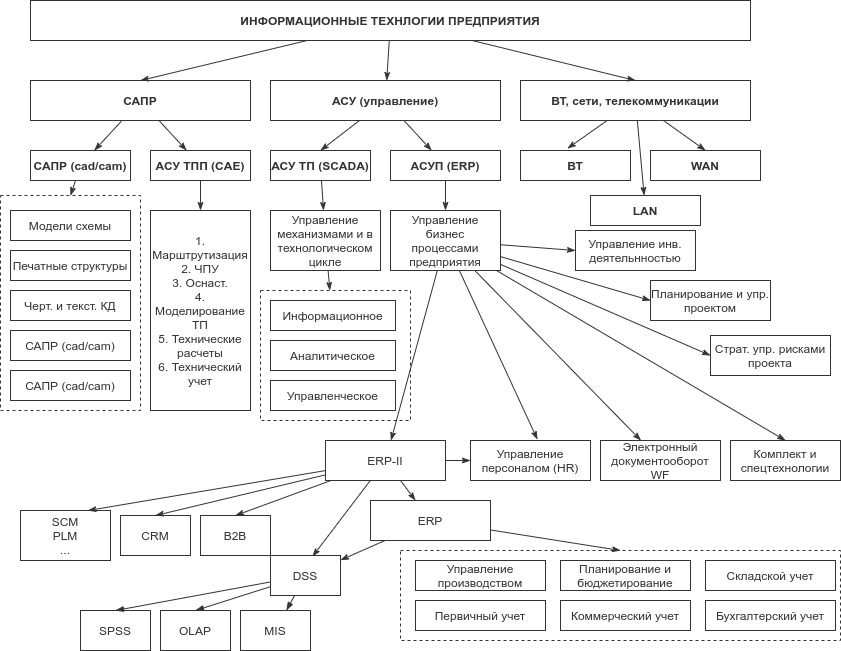
\includegraphics[scale=0.5]{DISSER-37.png}
    }
    \caption{Условная классификация информационных технологий предприятия}\label{fig:ITclass}
\end{figure}

Принципы проектирования программного обеспечения должны укладываться в следующие критерии, указанные на Рисунке~\cref{fig:principles}.  

\begin{figure}[ht]
    \centerfloat{
        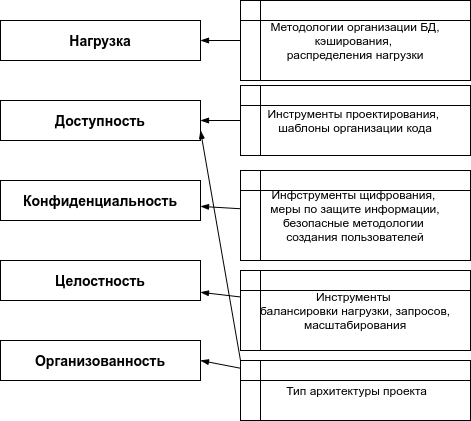
\includegraphics[scale = 0.8]{Dissertation/images/DISSER-52.png}
    }
    \caption{Принципы проектирования архитектуры программного обеспечения}\label{fig:principles}
\end{figure}

Автоматизированные системы управления, как понятие, появилось в СССР в 60-х годах двадцатого века в связи с внедрением вычислительной техники в организацию руководства СССР \cite[с.~38]{Yakovenko}. Для управления предприятием требуется контролировать все процессы, происходящие на предприятии, т.к. в зависимости от успешного ведения дел предприятия зависит его эффективность. Во многом кортролировать эффективность работы предприятия помогает внедрение автоматизированной системы управления, т.к. такая система позволяет следить за выполнением тех или иных процессов работы предприятия. Типовая автоматизация процессов предприятия включает в себя следующие направления:

\begin{enumerate}
	\item автоматизация процессов деятельности предприятия (например, бухгалтерский учет, управление персоналом, логистика, управление снабжением и т.д.),
	\item автоматизация основных технологических процессов предприятия,
	\item автоматизация процессов управления, процессов принятия решения, анализа, стратегического планирования деятельности предприятия.
\end{enumerate}

В целом, все предпрития условно можно разделить на 2 класса:
\begin{enumerate}
	\item предприятия с дискретным типом производства,
	\item предприятия с непрерывным производством.
\end{enumerate}

Единое информационное пространство предприятия состоит из совокупности всех баз, информационных банков данных, информационных технологий, информационно-вычислительных систем, телекоммуникационных сетей, протоколов безопасности, которые составляют единое информационное пространство для взаимодействия тех или иных субъектов технологического производства.

Единое информационное пространство условно можно представить согласно Рисунку ~\cref{fig:ITspace}.

\begin{figure}[ht1]
    \centerfloat{
       
       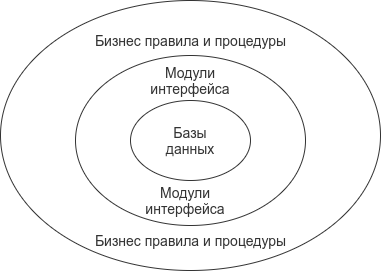
\includegraphics[scale=0.50]{DISSER-38.png}
    }
    \caption{Условная классификация информационных технологий предприятия}\label{fig:ITspace}
\end{figure}
Таким  образом, информационные технологии предприятия собирают в себе комплекс программно-аппаратных информационных средств составляющих интегрированную информационную среду: комплекс программно-ориентированных взаимосвязанных информационных подсистем, разрабатываемых для единого информационного пространства предприятия.

Интегрированная информационная среда, как единое информационное пространство предприятия представляется в следующем обобщенном виде, как на Рисунке ~\cref{fig:ITembeddedspace} \cite{ITclass}.

\begin{figure}[ht1]
    \centerfloat{
        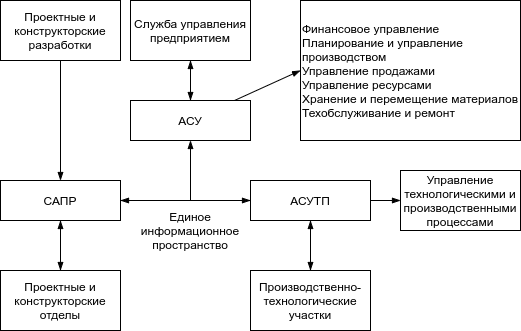
\includegraphics[scale=0.8]{DISSER-39.png}
    }
    \caption{Концептуальная модель интегрированной информационной среды}\label{fig:ITembeddedspace}
\end{figure}

Следующие компоненты составляют типовую интегрированную информационную среду:
\begin{enumerate}
	\item телекоммуникационная среда в составе коммуникационного программного обеспечения,
	\item средства организации коллективной работы сотрудников,
	\item информационные ресурсы (ERP системы, программное обеспечение управления документооборотом, информационая поддержка предметных областей, программное обеспечение анализа информации и поддержки принятия решения, программное обеспечение управления проектами),
	\item инфраструктура для организации информационной среды,
	\item система обучения персонала, система переподготовки кадрового персонала.
\end{enumerate}
Систематизируем общие типовые требования для проектированая интегрированной информационной среды предприятия:
\begin{enumerate}
	\item интеграция горизонтальная и вертикальная существующего программного обеспечения с новым функционалом,
	\item единство организационных, технических и технологических принципов построения информационной среды,
	\item единая парадигма обмена информации и передачи данных на основе различных физических носителях,
	\item соответствие международным и российским стандартам разработки программного обеспечения,
	\item обспечение доступа пользователей к базам данных и необходимым источникам информации,
	\item обеспечение информационной безопасности и многоуровневой защиты данных, обеспечение гарантии подлинности информации,
	\item средства коллективного доступа к информационной среде,
	\item применение принципа модульности при проектировании системы и ее состовляющих подсистем,
	\item внедрение сертифицированных решений и решений, соответсвующих стандартам,
	\item мониторинг инфорационных средств и решений,
	\item использование методологий для совершенствования внедренных технологий.
\end{enumerate}
Таким образом, при проектировании информационной среды требуется следующий аналитический базис для планирования работ: 
\begin{enumerate}
	\item реалистичная оценка действительности для планирования взаимодействия с информационной средой всех пользователей системы,
	\item единый центр принятия решений при планировании работ для согласованной работы всех субъектов взаимодействия информационной среды во избежании несогласованных с имеющимися в пользовании средств и инструментов информационной среды,
	\item полезный результат, получаемый от организации информации, информационной среды, информационного пространства,
	\item анализ лучших практик организации информационной среды, информационного пространства, внедренных на рынке,
	\item понимание целей информатизации конкретного объекта информатизации, понимание полезного результата с внедрения информатизации для объекта,
	\item транслирование внедренных технологий во внешних мир для развития рынка в этой области.
\end{enumerate}

Экспертная система на основе искусственного интеллекта, которая обрабатывает слабоструктурированную и трудно формализуемую информацию в некоторой предметной области, может интерпретировать и объяснять методы решения задач принятия решения. Экспертные системы способны анализировать и предлагать множество решений на основе некоторых параметрических критериев. Такие системы обрабатывают информацию на основе некоторых формализованных структуированных закономерностях логического вывода, в данной работе модулем выявления закономерностей выступает критерий максимума взвешенной информативности.

Элементами экспертной системы являются следующие модули блоки обработчики:
\begin{enumerate}
    \item база знаний — некоторое семантическое представление знаний, формализованных в виде базы закономерностей, построенной на основе отбора критерием максимума взвешенной инфрмативности по таблице каналов наблюдений на основе ТРИЗ методологии,
    \item блок логического выводе — блок, который моделирует механизм поиска закономерностей, на основе отбора каналов наблюдения и классификации на основе критерия максимума взвешенной информативности,
    \item блок интерпретаций — блок, который интерпретирует некоторое семантическое представление получаемых системой данных,
    \item блок формирования рекомендаций — данный блок формирует рекомендации.
\end{enumerate}

Таким образом, системы поддержки принятия решения, основанные на экспертных системах, главным образом, опираются на модуль формирования закономерностей.

\section{Классы автоматизированных систем управления}\label{sec:ch2/sec1}
Классы автоматизированных систем управления:
\begin{enumerate}
	\item ОГАС - общегосударственная автоматизированная система сбора, хранения и обработки данных для задач учета, планирования и управления народным хозяйством страны в целом,
	\item ОАСУ — отраслевая автоматизированная система управления, объектом которой является определенная отрасль народного хозяйства страны;
	\item АСУП — автоматизированная система управления предприятием на основе применения вычислительных систем и экономико-математических методов для решения основных задач производственно-хозяйственной деятельности. Цель АСУП заключается в обеспечении неуклонного увеличения выпуска продукции путем непрерывного повышения технического и организационного уровня производства;
	\item АСУТП — автоматизированная система управления технологическим процессом, предназначенная для выработки и реализации управляющих воздействий на технологический объект управления (ТОУ) в соответствии с принятым критерием оптимальности..
\end{enumerate}
Рассмотрим внимательнее информационные потоки и процессы, которые отображают деятельность объекта автоматизации для:
\begin{enumerate}
	\item автоматизированных систем управления предприятием,
	\item автоматизированных систем управления технологическим процессом.
\end{enumerate}

Автоматизированная система управления состоит из множества подсистем, в основном они раздеделяются на две модели:
\begin{enumerate}
	\item нормативная модель управления,
	\item модель управления текущими состояниями.
\end{enumerate}

Нормативная модель управления представляет собой модель планирования ресурсов для обеспечения работы процессов на производстве:
\begin{enumerate}
	\item коэффициенты расчета показателей использования материально-технических средств,
	\item коэффициенты расчета показателей использования энергетических ресурсов,
	\item коэффициенты расчета показателей трудоемкости использования деталей,
	\item коэффициенты расчета показателей произвоительности труда,
	\item коэффициенты расчета показателей использования финансовых фондов,
	\item коэффициенты расчета показателей экономической эффективности.
\end{enumerate}

Модель текущих состояний расчитывается на основе текущей информации, получаемой в результате выполнения функции учета текущих состояний и планируемыми показателями.

Таким образом, для принятия решений расчитывается дифференциал между текущей информацией, получаемой в результате выполнения функции учета текущих состояний и планируемыми показателями.

Автоматизированные системы управления предприятием состоит из двух основопологающих подсистем:
\begin{enumerate}
	\item управляемая подсистема,
	\item управляющая подсистема.
\end{enumerate}
Управляемая подсистема является объектом, а управляющая подсистема является субъектом. В управлемой системе главными объектами иныформатизации выступают материальные и энергетические потоки. В управляющей системе главными объектами выступают информационные процессы и потоки.

В автоматизированных системах управления предприятием основной целью работы системы является предоставление информации для принятия решений в управлении предприятием. В автоматизированных системах управления технологическим процессом основной целью является контроль за выполнением технологического процесса.

Функциональные подсистемы АСУП можно разделить на следующие категории :
\begin{enumerate}
	\item управление технической подготовкой процессов производства,
	\item планирование экономических и технических производств,
	\item оперативное управление процессами основного производства,
	\item управление материальными ресурсами,
	\item управление бухгалтерской и финансовой документации,
	\item управление кадровым персоналом,
\end{enumerate}
Управляющая подсистема управляет соответвующим объектом: функциональной подсистемой.
Автоматизирования подсистема технико-экономического планирования создается для прогнозирования развития производства:
в своем составе типовая подсистема решает следующие задачи:
\begin{enumerate}
	\item расчет оперативных планов-графиков, регламентирующих выпуск продукции в соответствии с материальными, техническими, экономическими и производственными возможностями, 
	\item определение возможностей наращивания производства согласно оценке темпов расширения производства,
	\item расчет и формирование планов выпуска продукции.
\end{enumerate}
Уровень детализации прогнозов определяется периодом прогнозирования. Существуют следующие виды типовых прогнозов в подсистемах технико-экономического планирования :
\begin{enumerate}
	\item производственно-стратегический прогноз,
	\item планирование выпуска на относительно большие промежутки времени,
	\item прогнозы производственного цикла.
\end{enumerate} 
Целью подсистемы технико-экономического планирования:
\begin{enumerate}
	\item определение основных напрвлений развития производства,
	\item определение объемов, сроков, ресурсов и т.д. для слежением за показателями производства,
	\item определение потребности в трудовых, метариеальных и финансовых ресурсов,
	\item определение результатов производственно - хозяйственной деятельности производства.
\end{enumerate}
Автоматизированая система управление технологическими процессами создается для организации технологической подготовки производства. Процессы технологической подготовки производства представляют собой следующее: это некоторое множество мероприятий, которые отвечают за технологическую подготовки производства, необходимых для выпуска заданного плана производства.
Основные функции технологической подготовки производства:
\begin{enumerate}
	\item разработка технологических процессов,
	\item проектирование и изготовление средств технического и технологического производства,
	\item организация процессов технологического производства.
\end{enumerate}
Основными задачами системы являются:
\begin{enumerate}
	\item предоставление информационных ресурсов для организации освоения производства новых изделий существующего образца,
	\item предоставление информационных ресурсов для организации создания новых изделий.
\end{enumerate}
Типовые процессы в автоматизированных системах управления технологическими процессами являются:
\begin{enumerate}
	\item измерение параметров технологического производства,
	\item измерение темпов технологического производства,
	\item измерение девиантности и отклонений от параметров производства,
	\item измерение процессов согласно командам оператора.
\end{enumerate}
Функции, которые подвергаются автоматизации:
\begin{enumerate}
	\item определение режимов технологического производства,
	\item формирование управляющих воздействий режимов технологического производства,
	\item управление математической моделью и параметрами технологического производства,
	\item регистрация технологических и экономических показателей технологического производства,
	\item распределение материальных, энергетических, кадровых потоков для задач обеспечения необходимого режима технологического производства,
	\item распределение ремонтных мероприятий между технологическим производством,
	\item распределение учебных мероприятий технологического производства,
	\item распределение плановых графиков и сменно-суточных работы для технологического производства.
\end{enumerate}
АСУТП различает в среднем пять видов режимов работы:
\begin{enumerate}
	\item режим сбора и обработки информации,
	\item рекомендательный режим,
	\item режим контроля и управления,
	\item режим непосредственного управления посредством цифрового манипулятора,
	\item иерархические системы управления.
\end{enumerate}

Режим сбора и обработки данных состоит из отчетов аналитической информации, которая поступает после сбора и обработки данных с технологического производства. Такие измерения могут проводится посредством системы датчиков, измерителей, специальных приборов, которые имеют способность собирать информацию с технологического производства и его процессов. Главной задачей данного режима является предоствление отчетов  в виде аналитической информации. Все результаты зачастую сохраняются в реестр или спецальный архив.
Режим рекомендательный главной задачей ставит формирование рекомендаций по:
\begin{enumerate}
	\item выбору подходящего режима работы технологического производства при заданных параметрах,
	\item определению управлеющих воздействий по переменным возделйствия на процесс технологического производства,
	\item определение локальных регуляторов процессов технологического производства.
\end{enumerate}
Режим контроля и управления состоит, в общем случае, из двух уровневой иерархической модели:
\begin{enumerate}
	\item нижнгий уровень отвечает за управление локальными регуляторами процессов технологического производства,
	\item верхний уровень отвечает за контроль параметров состония технологического процесса посредством сбора информации с датчиков контроля параметров.
\end{enumerate}

Режим непосредственного управления посредством цифрового манипулятора отвечает за формирование управляющих воздейством через ЭВМ, соединенную непосредственно с управляемым объектом.
Иерархические системы управления - система, состоящая из множества уровней подсистем, находящихся в соподчинении.
Первый уровень представляет собой подсистему, которая непосредственным образом управляет технологическим процессом или технологическими операциями.
Второй уровень представляет собой подсистему, которая осуществляет расчет и оперативную корректировку режимов технологических операций или процессов.
Третий уровень представляет собой центральную управляющую подсистему, которая осуществляет расчет, корректировку технологического режима всего процесса в целом.

Каждая подсистема имеет соответствующую ей ЭВМ, которая работает в одном из четырех описанных выше режимов.

\subsection{Типы транзакционных систем}\label{sec:ch2/sec1/sub1}

Система должна обладать следующими свойствами:
\begin{enumerate}
	\item сложность,
	\item делимость,
	\item целостность,
	\item многообразие элементов системы и различие их природы,
	\item структурность,
	\item адаптивность,
	\item интегрируемость. 
\end{enumerate}
Системы можно классифицировать согласно типам транзакций, которые происходят в системе.
Информационные потоки в транзакционных системах чаще всего классифицируются по типу хранения и обработки информационного потока данных. Классифицируем данные по следующим признакам:
\begin{enumerate}
	\item данные по деталям, чаще всего обработка элементарных данных,
	\item агрегированные данные, чаще всего суммирование по некоторым измерениям,
	\item метаданные, т.е. данные, которые могут описывать некоторые конфигурационные действия над данными (обстоятельства использвания данных).
\end{enumerate}
Данные образуют некоторый информационный поток, который может быть разделен по следующим направлениям:
\begin{enumerate}
	\item входной поток,получаемый системой при обработке (источником информации может служить любой объект),
	\item потоки сообщений, которые образуются в результате работы деловой логики взаимодействия объектов,
	\item архивные потоки, образуются из классов данных, спрос на выполнение которых стал устаревать,
	\item поток метаданных, данные, которые образовались за счет конфигурационных, логгированных, журналированных даннных,
	\item выходной поток, данные, которые получает пользователь на выходе из работы системы,
	\item обратный поток, данные, которые возвращаются в систему.
\end{enumerate}

\subsection{OLTP системы}\label{sec:ch2/sec1/sub2}
OLTP  транзакционная система - система обработки транзакций в реальном времени. Такие системы предназначены для ввода, обработки и структурирования информации в режиме реального времени. К таким системам обычно предъявляются следующие требования:
\begin{enumerate}
 	\item ограничения на обработку информации через реальное время, 
 	\item транзакционные модели данных должны быть сильно нормализованы,
 	\item в случае возникновения ошибок, транзакции должны возвращаться в исходное состояние, до момента начала совершения транзакции,
 \end{enumerate}
Компоненты исполнения транзакций являются частью компонентов нагрузки, исполнение которых ограничиваются строгими требованиями выполнения в определенный интервал времени. Более того, транзакции, после отработки постоянно обновляют базу данных. Для проектировании подобных систем следует учитывать следующие параметры и характеристики работы программного обеспечения:
\begin{enumerate}
	\item при проведении транзакции используется относительно небольшой объем данных,
	\item индексы в базу данных должны быть легко доступны для уменьшения времени обработки транзакции,
	\item система должна иметь относительно небольшой промежуток временного отклика,
	\item используются только нормализованные формы транзакционные модели,
	\item может поддерживать сложные транзакционные модели,
	\item модель обработки транзакций проектируется опираясь на требования по нижнему пределу ограничения пропускной способности информации.
\end{enumerate}
Таким образом, основная цель OLTP систем - предоставление доступа в ограниченном отрезке реального времени, в строгом соответствии с нижним пределом пропускной способности. Суть таких систем состоит в соблюдении ограничений по обработке транзакций в строго определенном режиме обработки: ограниченного во времени, ограниченного в нижнем пределе по нагрузке. Система должна обеспечивать вычислительную нагрузку в реальном времени в стогом соответствии с ограничениями по времени и пропускной способности. Система должна восстанавливаться  в исходное состояние транзакций в случае выявления ошибок обработки. Система должна обновлять значения базы данных после проведения каждой успешной транзакции. В системе основным критерием успешной работы является обработка транзакции за ограниченный период в реальном времени. Такие системы не ориентированы на сохранение данных, при надобности данные системы архивируются.

\subsection{OLAP системы}\label{sec:ch2/sec1/sub3}

OLAP системы - это системы, которые ориентированы на аналитическую обработку данных. Такие системы анализируют данные многомерные данные и чаще всего используются для построения анализа многомерных систем.

Цель таких систем, предоставление аналитических отчетов, поэтому фундаментом обработки данных становится база данных, основанная на фактах. Таблица фактов - является сердцем таких систем, правильно спроектированная таблица фактов, которых соблюдаются все правильно низкой связности и высокой группировки, обеспечивает быстрое время обработки запросов в таких системах. 

Таблица фактов содержит фактическую информацию о свойстве объектов или событий. Факты делятся по следующим признакам:
\begin{enumerate}
	\item факты о транзакциях, т.е. факты, хранящие информацию о конретных совершенных действиях, 
	\item факты о состояниях,
	\item факты о свойствах того или иного объекта,
	\item факты о событиях.
\end{enumerate}

Таблица фактов должна содержать один внешний составной ключ, который должен объединять первичные ключи таблиц измерений. В настощее время разработано множество стандартов для проектирования OLAP систем. В общем случае, архитектура таких систем относится к обработке анализа, хранения и преобразования данных в независимых слоях системы, абстрактно ограниченных программным кодом. Основная нагрузка в таких системах ложится на организацию составления аналитических данных, где могут применяться различными методы решения вывода и аггрегации инфомации: например, путем изоляции обращений к базе данных, через объектно реляционные запросы на высокоуровневом языке программирования, либо оптимизация запросов к базе данных. 
Подходы к проектированию систем будут рассмотрены более подробно далее в работе.

\subsection{Блокчейн системы}\label{sec:ch2/sec1/sub4}

Модель транзакций в блокчейн системах представляется собой линейно независимую модель распределенных транзакций и может быть задана в следующем виде, где $y_i, i=1,2, …, N$ отображает транзакции, проводимые за некоторый конечный промежуток времени :
\begin{equation}
	\begin{cases}
		y'_{1}= a_{11}(x)y_{1}+a_{12}(x)y_{1}+ ... + a_{1n}(x)y_{n}, \\
		y'_{2}= a_{21}(x)y_{1}+a_{22}(x)y_{1}+ ... + a_{2m}(x)y_{n} , \\
		... \\
		y'_{n}= a_{n1}(x)y_{1}+a_{n2}(x)y_{2}+ ... + a_{nm}(x)y_{n}. 
	\end{cases}
\end{equation}



В матричной форме эта система имеет вид $\bar{y'}(x)=A(x)y(x)$, где $A(x)$ – квадратная функциональная матрица коэффициентов 
$\bar{y}=(y_1(x),  y_2(x), …,y_n(x))^T$ – функциональный вектор—столбец неизвестных, $\bar{y'}=(y'_1(x),  y'2(x), ... ,y'_n(x))^T$ – функциональный вектор—столбец производных неизвестных системы уравнений.

Так как элементы матрицы $A$ являются постоянными функциями непрерывные на любом промежутке, то по теореме о структуре общего решения линейной однородной системы дифференциальных уравнений для того, чтобы найти общее решение $y_0= C_1\bar{y}_1(x)+C_{2}\bar{y}_{2}(x)+ ... + C_{n}\bar{y}_{n}(x)$ данной системы уравнений достаточно построить фундаментальную систему решений $\bar{y}_{1}(x), \bar{y}_2(x), ... , \bar{y}_n(x)$.

Как было предложено Л. Эйлером, будем искать решение $y(x)= \bar{g}e^{kx}$ т.е. линейную однородную систему дифференциальных уравнений с постоянными коэффициентами в виде произведения $n$ — мерного вектора $\bar{g} \neq 0$  на экспоненциальную функцию $e^{kx}$, где $k$  – некоторое число. Дифференцируя эту вектор—функцию и подставляя полученные функции в решаемое дифференциальное уравнение, получим $\bar{g}ke^{kx}=A\bar{g}e^{kx}$. 

Так как экспоненциальная функция строго положительна, то справедливо матричное уравнение $(A-kE)\bar{g}= 0$, которое позволяет найти собственные числа и собственные векторы матрицы коэффициентов $A$.Одним из методов вычисления собственных чисел матриц является решение уравнения $\bigtriangledown(A-kE) = 0$, которое следует из теоремы существования ненулевого решения линейной однородной алгебраической системы уравнений. Раскрывая определитель, получаем алгебраическое уравнение $k^n+ p_{n-1}k^{n-1}+p_{n-2}k^{n-2}+ ...+ p_0=0$   порядка $n$  относительно переменной $k$. В теории дифференциальных уравнений данное уравнение называют \textit{характеристическим уравнением} линейная однородная система дифференциальных уравнений. Для каждого собственного числа $k_i$  из матричного уравнения $(A-k_{i}E)\bar{g}=0$  находят некоторый собственный вектор $\bar{g}_i\neq0$. По построению вектор—функция $\bar{y}_i(x)= \bar{g}_{i}e^{k_{i}x}$  является одним из решений исходного линейной однородной системы дифференциальных уравнений.

Требования к блокчейн приложениям обобщены на Рисунке~\cref{fig:blockchhainreq}. Типовые архитектурные элементы  


\begin{figure}[ht]
    \centerfloat{
        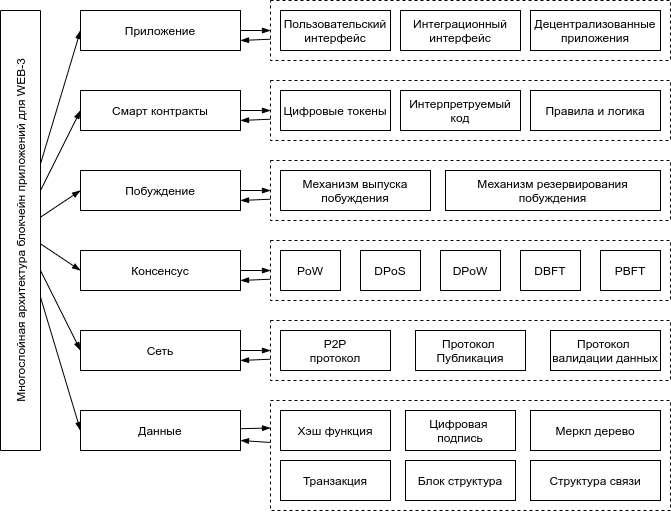
\includegraphics[scale=0.6]{Dissertation/images/DISSER-54.png}
    }
    \caption{Обобщенная архитектура в блокчейн приложениях согласно Индустрии 4.0}\label{fig:blockchhain}
\end{figure}

\begin{figure}[ht]
    \centerfloat{
        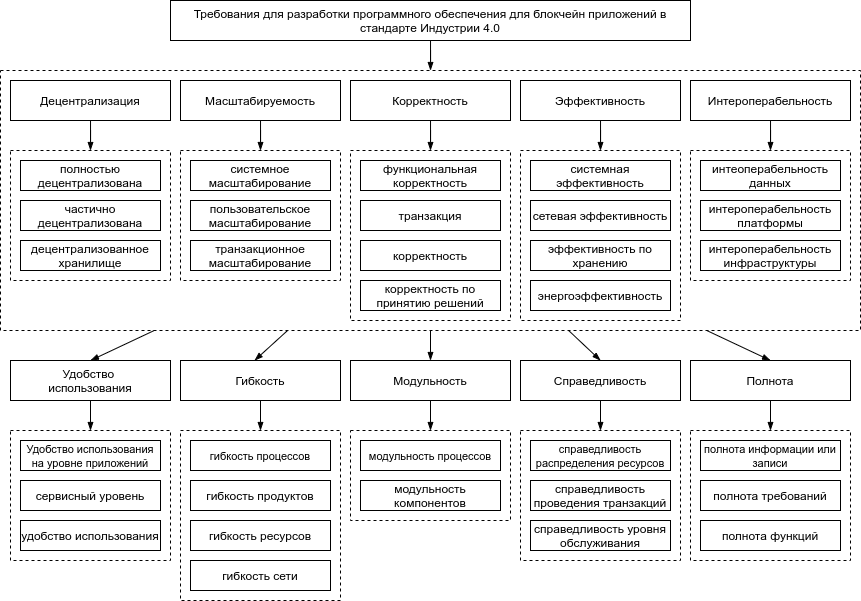
\includegraphics[scale=0.5]{Dissertation/images/DISSER-55.png}
    }
    \caption{Требования к блокчейн приложениям}\label{fig:blockchhainreq}
\end{figure}

\subsection{Высоковычислительные системы}\label{sec:ch2/sec1/sub5}


\subsection{Высоконагруженные системы}\label{sec:ch2/sec1/sub6}


\subsection{Типы предоставления доступа}\label{sec:ch2/sec1/sub7}

Системы автоматизированного управления могут быть разделены по следующим моделям предоставления доступа:
\begin{enumerate}
	\item SaaS модель предоставления доступа,
	\item PaaS модель предоставления доступа,
	\item IaaS модель предоставления доступа.
\end{enumerate}

\subsection{SaaS системы}\label{sec:ch2/sec1/sub8} 

SaaS система - система организации кода в виде предоставления доступа к программному обеспечению, как к услуги. 
Программное обеспечение системы SaaS обладает следующими ключевыми признаками:
\begin{enumerate}
    \item доступ к программному обеспечению, разработанному в соответствии с моделью программного обеспечения, как услуга, предоставляется удалённо по сетевым каналам и, как правило, через веб-интерфейс, кроме того, могут использоваться тонкие клиенты и терминальный доступ;
    \item программное обеспечение развёртывается в центре обработки данных в виде единого программного ядра, с которым работают все заказчики;
    \item обслуживание и обновление программного обеспечения выполняется централизованно на стороне поставщика приложения, предоставляемого как услуга (SaaS).
\end{enumerate}

\subsection{PaaS системы}\label{sec:ch2/sec1/sub9}
PaaS система предоставляет доступ к программному обеспечению через платформу. Платформа, предоставляется, как услуга. Чаще всего модель предоставляется, как облачный сервер с набором реализованного функционала или инструментария в аренду под конкретные цели. Модель, предоставляется за счет облачных вычислений, реализованных на облачном сервере. Функционал информационно-вычислительной инфраструктуры, включая вычислительные серверы, серверы, системы хранения, целиком управляется провайдером услуг. 


\subsection{IaaS системы}\label{sec:ch2/sec1/sub10}
IaaS системы - это такой тип систем, который предоставляет инфроструктуру как сервис. Чаще всего данные размещаются на облаке или в гибридном доступе, функционал по разработке инфраструктуры предоставляется по подписке. С помощью модели IaaS инфраструктура располагается на облаке, как набор сервисов.
С помощью модели IaaS компании могут частично или полностью переместить в облако локальную инфраструктуру центра обработки данных, где ее обслуживанием и управлением занимается поставщик облачных сервисов. К числу таких экономически эффективных элементов инфраструктуры могут относиться вычислительные и сетевые ресурсы, оборудование для хранения данных, а также другие компоненты и программное обеспечение. 
В рамках стандартной модели IaaS компании любого размера используют различные сервисы, такие как вычислительные ресурсы, хранилище и базы данных, предоставляемые поставщиком облачных решений. Поставщик услуг предоставляет эти сервисы путем размещения оборудования и программного обеспечения в облаке. Компании при этом не требуется приобретать собственное оборудование, заниматься его администрированием и отводить под него место в своих центрах обработки данных. А затраты она несет по модели «оплата по мере использования». Если компании нужно меньше ресурсов, общие затраты на них снижаются. А по мере роста компания может за считаные минуты предоставить сотрудникам дополнительные вычислительные ресурсы и другие технологии.
\section{Постановка задачи проектирования архитектуры автоматизированных систем управления, основные ограничения и допущения}\label{sec:ch2/sec2}

При проектировании системы основопологающими принципами проектирования является соблюдение следующих стратегий:
\begin{enumerate}
	\item миссия и видение проекта,
	\item руководящие принципы,
	\item цели, задачи, стратегии,
	\item архитектура ИТ.
\end{enumerate}

Соблюдение следующих тактик:
\begin{enumerate}
	\item политики и правила,
	\item ИТ - стандарты,
	\item Процедуры,
	\item Руководства.
\end{enumerate}

Изобразим данную парадигму проектирования в следующем виде, согласно Рисунку~\cref{fig:StrategyM}.
\begin{figure}[ht1]
    \centerfloat{
        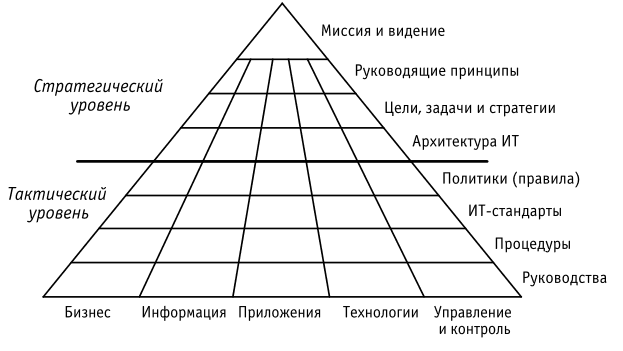
\includegraphics[scale=0.7]{DISSER-40.png}
    }
    \caption{Основопологающие принципы проектирования}\label{fig:StrategyM}
\end{figure}

Данный рисунок показывает, что руководящие принципы при проектировании системы накладывают ограничения на конкретные принципы, тактики и стратегии. Перейдем к рассмотрению ТРИЗ в разделе 2.3.1 подробнее далее. Но сейчас остановимся на более подроьном рассмотрении приципов проектирования архитектуры. 
\subsection{Принципы проектирования}\label{sec:ch2/sec1/sub11}
 Самыми главными элементами описания информационной архитектуры проектирования ИТ системы являются следующие:
 \begin{enumerate}
 	\item Миссия и видение.
 	\item Руководящие принципы.
 	\item Цели, задачи и стратегии.
 	\item Архитектура информационной технологии.
 	\item Политики и правила.
 	\item ИТ - стандарты.
 	\item Процедуры.
 	\item Руководства и рекомендации (best practices).
\end{enumerate}

Существует два основных направления проектирования архитектуры : 
\begin{enumerate}
	\item на основе принципов,
	\item на основе моделей.
\end{enumerate}

В архитектурной методике, разработанной Togaf\cite{Togaf}, эти два напрваления комбинирует в следующий принцип: придерживаться деклараций и следованию принципов, описывая состояния архитектуры в виде моделей, описывающие отдельные домены представлений.
Согласно представлению NASCIO (Национальная ассоциация руководителей информационных служб штатов США), влияние различных компонентов друг на друга представимо в следующем виде на Рисунке~\cref{fig:NASCIO}.
\begin{figure}[ht1]
    \centerfloat{
        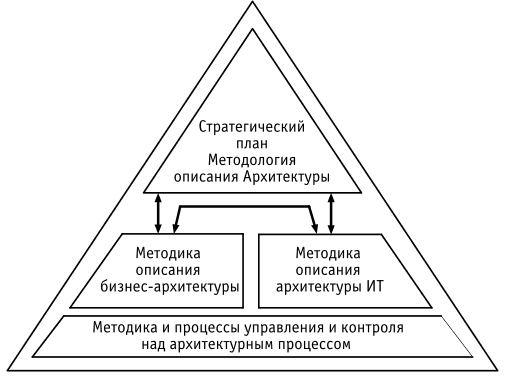
\includegraphics[scale=0.7]{DISSER-41.png}
    }
    \caption{Влияние различных компонентов друг на друга согласно модели NASCIO}\label{fig:NASCIO}
\end{figure}

Таким образом, архитектура представляет собой целостный процесс, который основан на ключевых стратегиях. Ключевые стратегии в свою очередь связывают бизнес, организацию, производство, информацию, прикладные системы, технологические процессы.
Интересным определением архитектуры является выражение Билла Гейтса в его книге "Бизнес со скоростью мысли", в которой он сравнивает архитектуру с электроной нервной системой предприятия. В его понимании, архитектура, подобно нервной системе, есть совокупность электронных процессов, которая должна адекватно воспринимать мир и реагировать на изменения, происходящие в нем.  

Архитектура программного обеспечения автоматизированной информационной системы представляет собой взаимосвязанную систему компонентов и модулей, которые стремятся обеспечить решение некоторой поставленной задачи автоматизации. Архитектура состоит из множества технических решений, которые можно комбинировать некоторым способом, архитектура допускает множество технических реализаций путем выбора различных компонентов архитектуры и методов взаимодействия между ними. В данной работе представлена модель архитектуры т.е. модель Библиотекаря для проектирования высоконагруженных автоматизированных информационных систем, с выполнением необходимых свойств, описанных выше.  
Перечислим типовой перечень сервисов и служб, необходимых для проектирования автоматизированной информационной системы:
\begin{enumerate}
	\item организация хранилища данных;
	\item организация обработки данных;
	\item формирование деловых функций объекта автоматизации;
	\item создание пользовательского интерфейса;
	\item разработка каналов обмена и передачи информации для интеграции со сторонними сервисами или ресурсами.
\end{enumerate}
Основополагаюшими понятиями в проектировании архитектуры для автоматизированной системы управления являются следующие объекты:
\begin{enumerate}
	\item ресурсы проектируемой информационной системы,
	\item процессы проектирумой информационной системы,
	\item состояния процессов проектируемой информационной системы,
	\item производительность процесса проектируемой информационной системы,
	\item информационная нагрузка на процесс проектируемой информационной системы,
	\item информационный поток на процесс проектируемой информационной системы,
	\item информационный объем на процесс проектируемой информационной системы,
	\item риск потери информации в процессах проектируемой информационной системы,
	\item производительность информационной системы в целом.
\end{enumerate}
Не менее важным вопросом при проектировании информационной системы является определение \textbf{объектов, которые будут структурировать данные}.


Процессы в информационной системе охарактеризуем, как следующие виды действий в типовой информационной системе на обобщенном уровне:
\begin{enumerate}
    \item действие введения информации из внутреннего ресурса,
    \item действие введения информации из внешнего ресурса,
    \item действие обработки информации во внутреннем ресурсе,
    \item действие обработки информации во внешнем ресурсе,
    \item действие по хранению информации во внутреннем ресурсе,
    \item действие по хранению информации во внешнем ресурсе,
    \item действие по передаче информации во внутренний ресурс,
    \item действие по передаче информации во внешний ресурс.
\end{enumerate}


Впоследствие, при проектировании информационной системы, действия в конкретной деловой логике можно категоризировать согласно видам действий, описанным выше.

Формализуем данную задачу. 

Пусть множество типов информационных систем, описываемых пользователем как  $U=\{u1,u2,...,un\}$, множество объектов, т.е. предлагаемых архитектур $P=\{p1,p2,...,pm\}$, весовая матрица  $R=ri,j$ размера $nxm$,  $i\{1...n\},j\{1...m\}$. $N$ - желаемое количество рекомендаций, которые нужно получить от системы. Набор типов информационных систем состоит из объекта, описываемого как набор некоторых характеристик, которые должны быть заполнены пользователем. Набор характеристик состоит из следующих обязательных пунктов для заполнения с множеством возможных решений, которые необходимо принять:
\begin{enumerate}
\item количество транзакций в секунду на чтение,
\item количество транзакций в секунду на запись,
\item количество пользователей,
\item требования к дальнейшей масштабируемости,
\item функциональные требования,
\item типы объектов в системе.
\end{enumerate}
Требуется найти: для описываемого набора типов информационных систем $u$, найти $N $- мерный вектор $p_{i1},p_{i2},...,p_{iN}$, где архитектура $p_{ik},k\in N$  еще не оценены экспертами, т.е. в матрице описания транзакций есть пустое место $r_i,i_k$, где эти архитектуры наиболее точно соответствуют базе конюнкционных закономерностей, то есть классам, здесь $r_i,i_k$ является наибольшим. Алгоритмы, необходимые для решения этой задачи, могут быть самыми разными и использовать разные входные данные. Некоторые из них генерируют рекомендации только на основе данных об известных матрицах описания транзакций или на заранее описанных известных продукционных правилах. Другие используют дополнительные характеристики, используют матрицы описания транзакций, чтобы определить, какие из этих характеристик наиболее точно соответствуют предпочтениям пользователя, а затем выбирают альтернативы с этими характеристиками.

\section{Решение проблемы проектирования устойчивой архитектуры программного обеспечения автоматизированной системы управления}\label{sec:ch2/sec2}
Для решения проблемы проектирования устойчивой архитектуры программного обеспечения автоматизированной системы управления следует внимательно рассмотреть соответсвующие параметры, требуемые для конфигурации архитектуры программного обеспечения:
\begin{enumerate}
	\item вычислительные ресурсы,
	\item скорость обработки данных,
	\item время обработки данных,
	\item объем данных,
	\item нагрузка пользовательская,
	\item размер объектов, структурирующие данные,
	\item устойчивость системы, 
	\item надежность системы,
	\item качество системы,
	\item информационная безопасность объектов системы,
	\item удобство эксплуатации системы,
	\item удобство создания системы,
	\item удобство ремонта,
	\item адаптация, универсальность,
	\item сложность разработки,
	\item сложность контроля и измерений,
	\item степень автоматизации,
	\item произвеодительность.
\end{enumerate}


Операция назначения каждому параметру значения переменой называется каналом наблюдения.

Система может быть описана в следующем виде:

\begin{equation}
    \label{eq:equation29}
    S =  (X, T, R, Z ) ,
\end{equation}

где $ X $  — множество переменных, 

$T$ — множество параметров, 

$R$ — отношения на множества $X$ и $T$, 

$Z$ — цель исследований т.е. решение проблемы проектирования устойчивой архитектуры программного обеспечения автоматизированной системы управления.

Данная система задается на множестве допустимых значений перемнной $ X = [X_{n}, i={1,N}] $, переменная изменяется в соответствии с $ X_{n} ={1,N}$, $[X_{n, k}, k = {1,N}]$. Вектор состояний системы задается в виде зафиксированного значения всех перемнных относительно одного значения параметра:

\begin{equation}
    \label{eq:equation30}
    C_{i} = [\alpha_{1,k_{1}}, X_{2,k_{2}}, ..., X_{N, k_{N}}] ,
\end{equation}

Возможные состояния множества описываются в виде вектора: $ C = [C_{i} , i={1,|C|}]$. Вектор образует полное множество состояний, 
где $|C| = \prod k_n$.

\subsection{ТРИЗ теорема для решения проблемы проектирования устойчивой архитектуры программного обеспечения автоматизированной системы управления}\label{sec:ch2/sec2/sub1}

При проектировании методологии нахождения подходящих по тем или иным критериям оценки альтернатив необходимым условием решения является определения компромисса. Для поиска компромисса выделяют противоречия ~\cite{trisonlinepetrov}. Для решеия данной задачи возпользуемся следующими постулатами ТРИЗ теоремы ~\cite{trisonlinepetrov, altshuller}:

\begin{enumerate}
	\item При решении задач и развитии систем необходимо использовать законы развития технических систем.
	\item  Любую изобретательскую задачу можно классифицировать, и в соответствии с видом задачи подбирается вид решения.
	\item  Для решения сложных изобретательских задач необходимо выявить и разрешить противоречие, находящееся в глубине задачи.
\end{enumerate}

Согласно доработанной методологии ТРИЗ - АРИЗ Универсал 2010 ~\cite{ariz-2010} решение задачи состоит из следующих шагов , представленных на Рисунке ~\cref{fig:ariz-1}:

\begin{enumerate}
	\item уточнение формулмрования задачи, включая выявление противоречий в задаче, при необходимости используется функциональный и другие виды анализов задачи,
	\item анализ функций и функционально-ориентированный поиск ,
	\item противоречия требований и приемы их разрешения,
	\item элепольная модель и стандарты решения изобретательских задач,
	\item анализ противоречий свойств и мобилизация ресурсов,
	\item оценка решения, изменение и переформулировка задачи, выявление вторичных задач, развитие и обобщение найденного решения,
	\item накопление идей, которые возникают в ходе анализа задачи и поиска решения,
	\item дополнительный анализ.
\end{enumerate}


\begin{figure}[ht]
    \centerfloat{
        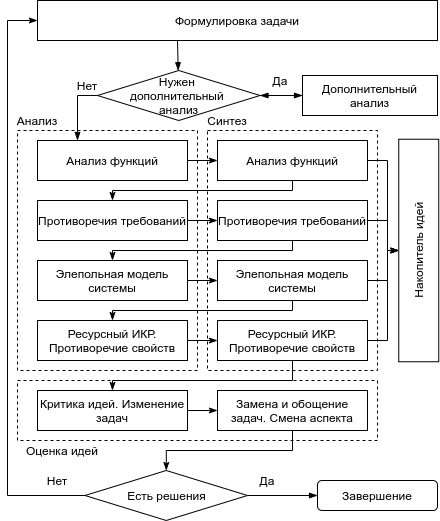
\includegraphics[scale=0.7]{DISSER-42.png}
    }
    \caption{АРИЗ Универсал 2010}\label{fig:ariz-1}
\end{figure}

Ключевые шаги АРИЗ Универсал 2010, состоят из следуюших этапов, указанных на Рисунке ~\cref{fig:ariz-2}:

\begin{enumerate}
	\item анализ задачи,
	\item синтез задачи,
	\item критическая оценка предлагаемого альтернативного решения.
\end{enumerate} 


\begin{figure}[ht]
    \centerfloat{
        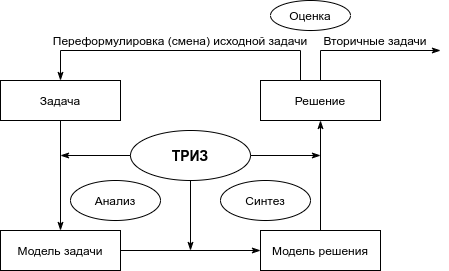
\includegraphics[scale=0.7]{DISSER-43.png}
    }
    \caption{АРИЗ Универсал 2010}\label{fig:ariz-2}
\end{figure}

Таким образом, таблица противоречий состоит из следующих каналов наблюдения и приложена к работе в Приложении ~\cref{app:B2}:

\begin{enumerate}
	\item вычислительные ресурсы (серверное оборудование, сеть, оборудование сопряженное, коммутация, техничесие средства ЭВМ, облачные ресурсы и т.д.),
	\item время обработки данных,
	\item скорость обработки данных,
	\item объем данных,
	\item количество запросов за единицу времени,
	\item количество пользователей/потребителей информации,
	\item нагрузка на систему,
	\item размер объектов, структурирующие данные,
	\item устойчивость элементов системы (пго конкретным элементам),
	\item устойчивость всей системы в целом,
	\item количество элеметнов, структурируюшие данные в системе,
	\item качество элементов системы,
	\item качество всей системы,
	\item надежность элементов системы,
	\item надежность всей системы в целом,
	\item информационная безопасность элементов системы,
	\item информационная безопасность всей системы,
	\item удобство экспуатации системы,
	\item удобство эксплуатации элементов системы,
	\item удобство изготовления элементов системы,
	\item удобство изготовления всей системы,
	\item удобство ремонта элементов системы,
	\item удобство ремонта всей системы в целом,
	\item удобство обновления элементов системы,
	\item удобство обновления всей системы в целом,
	\item удобство сопровождения элементов системы,
	\item удобство сопровождения всей системы,
	\item адаптация элементов системы,
	\item адаптация всей системы в целом,
	\item сложность разработки элементов системы,
	\item сложность разработки системы,
	\item сложность контроля и измерений состояний процессов,
	\item сложность вычислений,
	\item сложность использования ресурсов, 
	\item сложность использования объектов, структурирующих данные,
	\item степень автоматизации системы,
	\item производительность.
\end{enumerate}

Таким образом, перечисленные каналы наблюдения будут использоваться, как основные параметры для обучения алгоритма классификации и поиска максимального значения функионала производительности.


\subsection{Параметрический критерий нагрузки на автоматизированные системы}\label{sec:ch2/sec2/sub2}
Рассмотрим параметрический критерий нагрузки на системы, основанный на следующем свойстве экспоненциального распределения плотности 
\begin{equation}
    \label{eq:equation20}
    f(t) = \frac{1}{T}e^{(-1T)}, T = \sqrt{D}  
\end{equation}

где $T$ - математическое ожидание экспоненциального закона;

$D$ - дисперсия, определяемая по зависимости ~\cref{eq:equation21}
\begin{equation}
    \label{eq:equation21}
    D = \int_0^{\infty} \mathrm \{\frac{(1-T)^2}{T}e^{-\frac{1}{T}}\,\mathrm{d}t    
\end{equation}

Рассмотрим случай, когда на систему действует два источника нагрузки: пользовательская нагрузка, состоящая из поступающего на обслуживание через веб-сервер множество запросов и запросы командной нагрузки от сторонних платформ, поступающие через интеграционные шлюзы. Запросы проходят через доменные имена и распределяются в балансировщиках нагрузки, которые направляют входящие запросы на один из множества серверов приложения, которые обычно являются зеркальными копиями друг друга, и отправляют ответ обратно пользователю. Любой сервер обрабатывает запросы одинаково, так что балансировщик занимается распределением заданий, чтобы никакой из них не был перегружен.
Таким образом, в момент старта работы приложений запросы между пользователями могут соревноваться за ресурсы информационной системы. Для описания этого процесса воспользуемся двух-параллельным марковским процессом ~\cref{eq:equation22}
\begin{equation}
    \label{eq:equation22}
    M = [A, h(t)]  
\end{equation}
                       (3)
где $ A = \{a_{w1},a_{w2}, a_{g1},a_{g2} \}$ - множество состояний, 

$a_{w1}, a_{g1}$ - стартовые состояния, 

$a_{w2}, a_{g2}$ - поглощающие состояния, 

$h(t)$ - полумарковская матрица;

Для определения времени ожидания процесса воспользуемся описанием вида ~\cref{eq:equation23}


\begin{equation}
    \label{eq:equation23}
    M = [A', h'(t)]  
\end{equation}

где $A' = AB$ - множество состояний;

$A = \{\alpha_1, \alpha_2, \alpha_3\}$ - подмножество состояний, моделирующее начало и окончания блужданий по полумарковскому процессу; 

$\alpha_1$ - стартовое состояние;

$\alpha_2$ - поглощающее состояние, моделирующее выигрыш второго субъекта; 

$\alpha_3$ - поглощающее состояние, моделирующее окончание ожидания первым субъектом окончания второго;

$B = \{\beta_1,\beta_2, \beta_3 \}$ - бесконечное множество состояний, задающих временные интервалы ситуаций завершения обслуживания вторым
 $h'(t) = \{h'_{m,n}(t)\}$ - полумарковская матрица, задающая временные интервалы процесса.


Представим плотность распределения времени наблюдения за системой посредством закона вырожденного распределения с некоторым математическим ожиданием  $T$   и  $\omega(t) = \delta(t - T)$ , который соответствует некоторому детерминированному процессу. Таким образом, плотность распределения времени ожидания завершения события $g(t)$, определяется согласно зависимости ~\cref{eq:equation24}:


\begin{equation}
    \label{eq:equation24}
    f_{\delta \rightarrow g(t)} = \frac{\eta(t)g(t+T)}{\int_T^{\infty} \mathrm {g(t)}}\,\mathrm{d}t}
\end{equation}

Математическое ожидание имеет вид ~\cref{eq:equation25}:
\begin{equation}
    \label{eq:equation25}
    T_{\delta \rightarrow g(t)} = \int_0^{\infty} \mathrm {t\frac{g(t+T)}{\int_T^{\infth} \mathrm{g(t)\,\mathrm{d}t}}}\,\mathrm{d}t}
\end{equation}

Критерий, основанный на определении времени ожидания для строго детерминированной связи между событиями, выражаемой - функции Дирака $g(t) = \delta(t - T)$, имеет вид:
\begin{equation}
    \label{eq:equation26}
    \varepsilon_{\omega} = \frac{t-T_{\delta\rightarrow\g}}{T}^2 
\end{equation}

где $T$ - математическое ожидание анализируемой плотности распределения времени между соседними событиями; 

$T_{\delta\rightarrow g}$- математическое ожидание плотности распределения $f_{\delta\rightarrow g(t)}, рассчитываемое по зависимости ~\cref{eq:equation24}.

Математическое ожидание распределения сигнала определяется по следующей зависимости 
\begin{equation}
    \label{eq:equation27}
    T_k = \int_0^1 \mathrm{tK(1-t)^{K-1}}\,\mathrm{d}t = \frac{1}{K+1}[время]
\end{equation}

Экспоненциальный закон, определяющий Пуассоновский поток событий 
\begin{equation}
    \label{eq:equation28}
    f_K(t) = (K+1)e^{[-(K+1)t]} [probtime]
\end{equation}

\subsection{Групповой критерий надежности работы системы}\label{sec:ch2/sec2/sub3}

Рассмотрим задачу анализа надежности системы с точки зрения моделирования группового отказа в системе. Представим, что модель работы в какой-то момент времени начнет отказывать в обслуживании, т.е. модули системы или некоторый функционал начнет давать сбой. Назовем такое поведение, как вероятность наступления группового отказа в системе. Модулями в системе выступает допустимое множество решений модели поддержки принятия решений.
Пусть вероятность наступления события отказа представляется в виде $k$ вершин надежных решений, где связи между вершинами, а также сами вершины определяют вероятность выхода из строя. Количество вершин ограничено от двух до произвольного значения. Таким образом, модель примет вид графа с вершинами, где ребра и вершины отображают вероятность наступления отказа. Вероятность наступления отказа в модели, отображающей множество решений   
При проектировании автоматизированной системы управления задача определения надежности работы системы является одной из важнейших задач. В эту задачу входят такие важнейшие аспекты работы системы, как \cite{ACSSt}:
\begin{itemize}
	\item совместимость между частями,
	\item готовность к масштабированию,
	\item приспособленность к модернизации,
	\item надежность в установленных целях и в заданных условиях применения,
	\item адаптивность для лостижения поставленных целей работы системы,
	\item меры безопасности и обеспечение безопасности работы системы в целом.
\end{itemize}

Рассмотрим данную задачу с точки зрения неориентированного графа в аспекте абстрактной модели проектируемой автоматизированной системы, где в зависимости от конкретной цели и типа системы будет видоизменяться некоторый набор параметров в модели оценки надежности работы системы. В литературе известны примеры исследования таких задач с помощью методологий, основанных на так называемых $k$ - терминальных надежностей, где определяется вероятность выхода из строя вершин и узлов графа. Однако, согласно выводам из \cite{groupotkazy} такие модели зачастую упускают вероятностный выход из строя надежных вершин, а также слишком упрощают реальные условия выхода из строя системы, что приводит к их неадекватности отражения реальности. 
Наиболее реалистичными сценариями отказов, согласно наблюдениями из \cite{groupotkazy}, являются отказы, которые приводят к цепочке отказов, происходящих одновременно или со временем. В общем смысле, ошибка состоит в рассмотрении события отказа , как независимого события.

В данной работе предлагается рассмотреть модель случайного графа.  
Каждое ребро или вершина может выходить из строя. При выходе из строя граф или вершина не восстанавливаются, т.е. удаляются из графа: при отказе работы вершины - удаляется вершина со веми инцидентными ей ребрами, при отказе работы ребра - удаляется ребро из графа. Распространение отказа в графе происходит последовательно, кратно минимально возможному интервалу времени. Допускается наличие некоторого порогового уровня распространения отказа в системе, после которого распространение отказа блокируется автоматически, например, посредством некоторого механизма безопасности. 
Таким образом, модель представляется в следующем виде:
отказы происходят каскадно, т.е. вероятность отказа элемента на $i$ - ом шаге зависит от того, какой конкретно элемент вышел из строя на предыдущем $i - 1$ - ом шаге.
На первом шаге элементы отказывают независимо. 


\section{Математическая модель системы логического вывода}\label{sec:ch2/sec3}

Для построения экспертной системы используются следующие алгоритмы:
\begin{enumerate}
	\item алгоритм построения семантического графа объектов и признаков для обучения модели по прецендентам,
	\item алгоритм построения коллекции решающих деревьев на основе таблицы противоречий,
	\item алгоритм классификации на основе алгоритма случайного леса для нахождения конечного вектора ответов для функционала производительности по каналам наблюдения из таблицы противоречий,
	\item алгоритм подбора рекоммендаций методом максимального правдоподобия функционала производительности на основе матричный разложений и  ортогонолизации параметров из каналов наблюдения модели.
\end{enumerate}

Обучающая выборка представляется в виде семантического графа, вершины которого состоят из объектов, которыми являются каналы наблюдения, а ребра представляют связь между каналами. Каждому каналу наблюдения проставляется оценка значимости первоначально случайным образом. 

\subsection{Поиск информативных конъюнкций как задача отбора признаков}\label{sec:ch2/sec3/sub1}
Для поиска информативных конъюнкций требуется приспособить один из методов отбора признаков. Вместо минимазации ошибки воспользуемся критерием макисимума информативности. Воспользуемся логическим алгоритмом классификации и информативной конъюнкцией. Синтез параметров, как признаков из графа параметров и ТРИЗ таблицы противоречий будет производится посредством поиска закономерностей. Задача стоит отделить линейно независимые параметры от линейно зависимых. Для этого из параметров графа будет строится система непересекающих множеств на основе древовидных структур данных. Основным принципом и критерием классификации будет критерий максимума информативности.

Каналы наблюдения задаются в виде функционалов нечеткой логики Мамдани. Каждому параметру соответсвет значение нечеткого функционала.

Представим модель в виде некоторой нелинейной системы:
\begin{equation}
    \label{eq:equation36}
    \[ \varphi(y(x)) = \left\{\begin{array}{ll} x_i, i   = 0,1, ...,  n,\textrm{,}\\ y_k = f_y(x_1,x_2,...,x_n), k = 1,2,...,q & \end{array} \right. \]
\end{equation}

Представим множество возможных значений в следующем виде:
\begin{equation}
    \label{eq:equation37}
    U = \{u_j, u_{j+1},.., u_m\}
\end{equation}

где $u_j$ - оценка, которая проставляется в соответсвии с входной информацией в систему,

$m$ - мощность множества.

Решением задачи будет составление такого множества значений $Y*= \{y_1^*, y_2^*, ..., y_n^*\}$ на постившее множество $X* = \{x_1^*, x_2^*,...,x_n^*\}$. Таким образом, на множество, поступающих значений $X*$ формируется множство выходных значений $Y*$.
Для установления зависимости между объектами выразим эвристическую закономерность в виде обработки семантических лингвистических переменных. Для этого выразим объекты через некоторые терм множества:
\begin{equation}
    \label{eq:equation38}
    A = \{a_j, a_{j+1}, ..., a_m\}
\end{equation}
Данные семантические терм определяются на основе соотношения
\begin{equation}
    \label{eq:equation38}
    a_j = \sum_{p=1}^l\frac{\mu^{a_{j}(u^p_j)}}{u^p_j}
\end{equation}

$\mu^{a_{j}(u^p_j)}$ - степень принадлежности,

$u^p_j$ - объект принадлежности.

Степень принадлежности определяется на основе рангов принадлежности и определяется на основе соотношений следующей системы:
\begin{equation}
    \label{eq:equation40}
    \[ R(\mu) = \left\{\begin{array}{ll} \frac{\mu_1}{\r_1} = \frac{\mu_2}{\r_2} = ... = \frac{\mu_m}{\r_m}, i   = 0,1, ...,  m,\textrm{,}\\ \sum_{i=1}^m{\mu_i} = 1  & \end{array} \right. \]
\end{equation}
В соответствии с нормировкой находим:
\begin{equation}
    \label{eq:equation41}
    \[ R(\mu) = 
    \left\{\begin{array}{ll} 
    \mu_{n-1} = (1 + \frac{r_n}{r_{n-1}} + \frac{r_{n+1}}{r_{n-1}} + ... )^{-1} \textrm{,} 
    \\ \mu_{n+m} = (\frac{r_{n-1}}{r_n} + \frac{r_{n+1}}{r_n} + ... )^{-1}  & \end{array} \right. \]
\end{equation}

Получаемая матрица обладает следующими свойствами:
\begin{enumerate}
    \item транзитивность,
    \item симметричность,
    \item диагональность.
\end{enumerate}

На основании этих свойств выведем соотношение:
\begin{equation}
    \label{eq:equation42}
    s_{ij} = \frac{s_{kj}}{s_{ki}}
\end{equation}

На основе матрицы парных рангов составляется соотношение со значениями 9-ти бальной шкалы Саати 
На рисунке ~\cref{fig:ST} представлена 9-ти бальная шкала Саати.

\begin{figure}[ht]
    \centerfloat{
        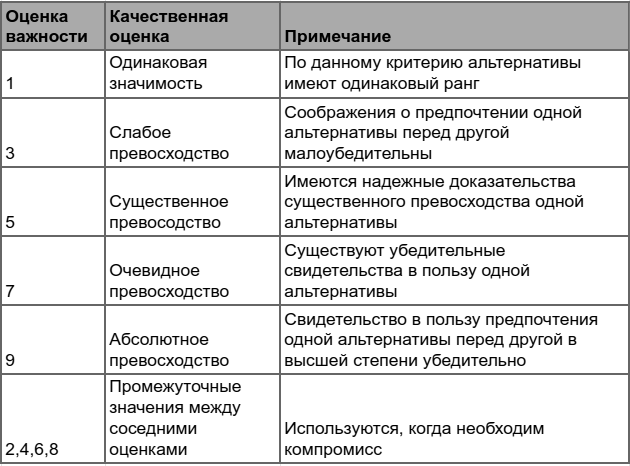
\includegraphics[scale=0.59]{Dissertation/images/APP-1.png}
    }
    \caption{9-ти бальная шкала Саати}\label{fig:ST}
\end{figure}

Приведем перечень функций принадлежности классов. Функция принадлежности к некоторому классу $s$ приведена в ~\cref{eq:equation43}.
\begin{equation}
    \label{eq:equation43}
    s(x,a,b,c) = \left\{\begin{array}{ll} 
    0, x\leq{a} \textrm{,} 
    \\ 2{\frac{x-a}{c-a}}^2, a\leq x\leq b    \\
    1 - 2{\frac{x-c}{c-a}}^2, b\leq x\leq c   \\ 
    1, x\geq c & \end{array} \right. \]
\end{equation}

где $b = \frac{a+c}{2}$.

Конъюнкционная закономерность интерпретируется на основе:
\begin{equation}
    \label{eq:equation44}
    (i): Q ; P; A \rightarrow B;S,F,N
\end{equation}

где $(i)$ - имя нечеткого  канала налюдения,

$Q$ - домен нечеткого канала налюдения,

$P$ - условия принятия, критерий принятия,

$A \rightarrow B$ - ядро конъюнкционой закономерности,

$B$ - результирующее заключение, следствие,

$\rightarrow$ - знак коньюнкционной секвенции,

$S$ - метод определения количественной истинности,

$F$ - коэффициент истины,

$N$ - ограничения конъюнкционного вывода.


База знаний в соответствии с представление в виде коньюнкционных правил образует совокупность множество, представимое в некоторой совокупности таблиц фактов.
Термы множества задаются с стандартной форме в виде логических отношений. База знаний задается в виде набора полей, объединенных некоторым логическим отношением, записанных в некоторой таблице совокупности фактов в виде графа, на основании которых выводится коньюнкционное правило.
Нечеткая база знаний может быть представлена в следующей виде в виде функции Мамдани:

\begin{equation}
    \label{eq:equation45}
    \bigcup_{p=1}^{t_k} [\bigcap_{i=1}^{n} \(x_i = a_j^{kp}\)]   \rightarrow  \bigcup_{p=1}^{t_k} [ \bigcap_{k=1}^{q} \(y_k = b_j^{kp}\)  ]
\end{equation}

где  $j = {1,2, ..., q}$, $k = {1,2, ..., q}$, $p = {1,2, ..., t_k}$

База знаний формируется в соответствии с Рисунком ~\cref{fig:KBase}. Структура матрицы знаний представлена с Рисунком ~\cref{fig:ST}.

\begin{figure}[ht]
    \centerfloat{
        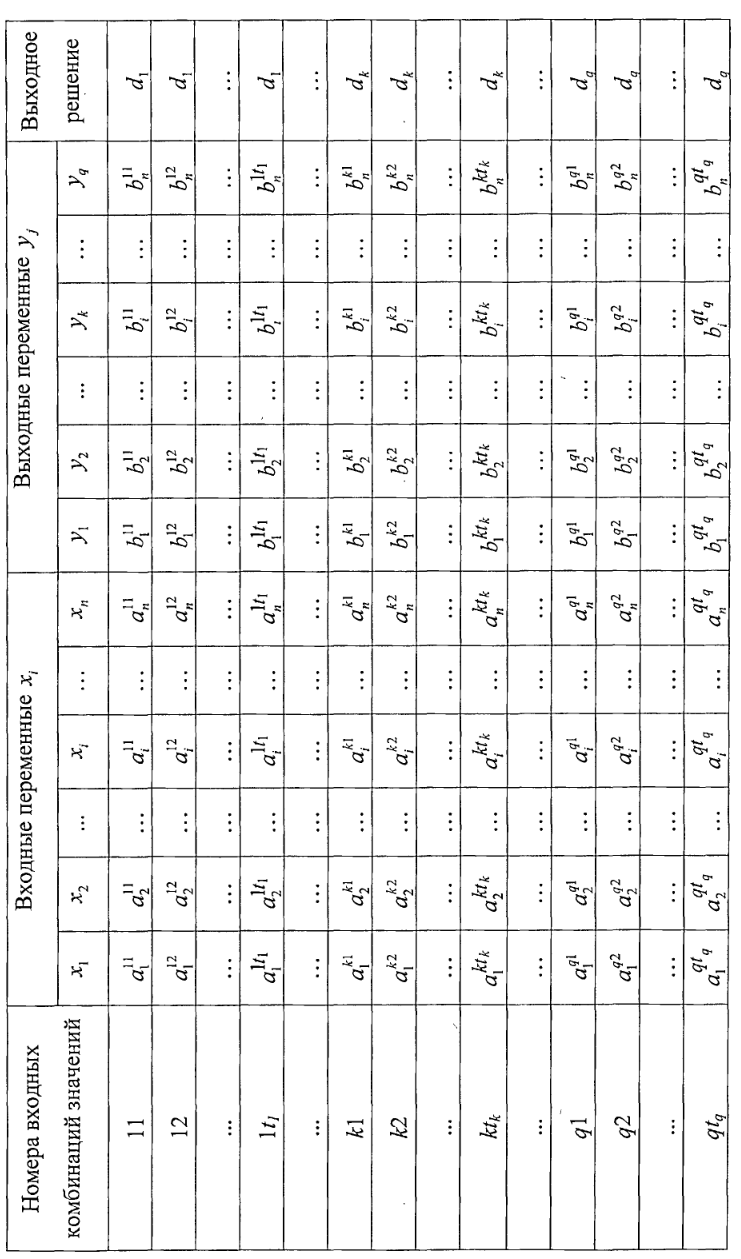
\includegraphics[scale=0.5]{Dissertation/images/DISSER-7.png}
    }
    \caption{Структура матрицы знаний}\label{fig:KBase}
\end{figure}

Система непересекающих множеств строится следующим образом:
\begin{enumerate}
	\item стоится дерево для множества, одно дерево соответсвует одному множеству,
	\item создается массив "родитель", на которого хранится ссылка, для корней дерева ссылка замыкается сама на себя,
	\item создается операция "$\rm make\_up$" добавляет новый элемент $ x $, помещая его в новое множество, состоящее из одного него,
	\item создается операция "$\rm union\_sets(x,y)$" объединяет два указанных множества (множество, в котором находится элемент $x$, и множество, в котором находится элемент $y$),
	\item создается операция "$\rm find\_set}(x)$" возвращает в каком множестве назодится объект - указанный элемент $x$.
\end{enumerate}

Если вызов $ {\rm find\_set}(x)$ для каких-то двух элементов вернул одно и то же значение, то это означает, что эти элементы находятся в одном и том же множестве, а в противном случае — в разных множествах.
Оценка асимптотики алгоритма будет логарифимческой на один запрос в среднем $ O (\log n)$ ~\cite{logn, tomaskormenm, kurtm, RobertEndreTarjan1, RobertEndreTarjan2}.

Алгоритм синтеза решающих деревьев правильно классифицирующих объекты по их признакам на классы является $NP$ - полной задачей.

В основе построения классификатора лежит прицнип индуктивного вывода логических закономерностей или индукции правил. 
Пусть $ \phi: X \rightarrow \{0,1\} $ некоторый предикат, который определяется на множестве объектов X. Предикат $ \phi $ является закономерностью и является неотемлимым атрибутом для построения закономерностей в процессе поиска правил по ваыборке и извлечения знаний из данных. К знаниям предъявляется особое требование -  интерпретируемость.

Всякая закономерность может классифицировать только некоторую часть объектов. Для того, чтобы классифицировать любые объекты требуется получить объединение закономерностей в некоторую композицию.  

Для поиска конъюктивных закономерностей в модели используется алгоритм построения логической классификации с помощью решающего дерева. Деревом называется конечный граф с множеством вершин $ V $, которые не содержат циклы и имеет вершину $ v_{0} \in V$, в которую ни одно ребро не входит. Такая вершина называется корнем дерева. Вершина, которая не имеет выходящих ребер, называется терминальной или листом. Остальные вершины называются внутренними.

Объект $x$ доходит до вершины $v$ при условии, что выполняется конъюнкция K_{v}(x) всех предикатов внутренних вершин дерева на пути от корня $v_{0}$ до вершины $v$. Пусть $T$ - множество всех терминальных вершин. Множества объектов $\Omega_{v} = {x \in X }$ выделяется терминальными конъюкциями $v \in T$. Объекты $x$ попарно не пересекаются, объединение объектов совпадает со всем пространством $X$.

Пусть $X $ - пространство объектов, $Y = \{1,2, ..., M\}$ - множество классов. Тогда, целевая зависимость $X $ от $Y$ задается в следующем виде: $X^{l} = (x_{i},y_{i})^l_{i=1}, y_{i} = y^*(x_{i})$. Алгоритм классификации $ a: X \rightarrow Y $ аппроксимирует $y^*$ на всем множестве $Y$.

В общем случае, ансамбль решающих деревьев строится на основе критерия
Введем значение количества объектов, как $N$, а количество признаков $ D $. Пусть $L$ - число отдельных моделей в ансамбле. Для каждой отдельной модели $l$ выбирается $dl (dl < D)$, такой дифференциал представляет собой число признаков для $l$. Для всех моделей, по умолчанию, выбирается одно значение $dl$. Для каждой отдельной модели $l$ создается обучающая выборка посредством выбора $dl$ признаков из $D$ для обученяи модели. Далее, для применения модели к новому объекту следует объединить результаты отдельных $L$ моделей путем мажоритарного голосования:

\begin{equation}
    \label{eq:equation29}
    a(x) = argmax_{\substack{ y \in Y
  }} \sum_{\substack{
   v \in V \\
   Cv = y
  }} 
 K_{v}(x)
\end{equation}

\subsection{Критерий максимума информативности}\label{sec:ch2/sec3/sub3}

Предикат $\phi$ называется информативным, если он отбирает наибольшее количество объектов одного классов $c \in Y$, к которому принадлежит, по сравнению с объектами другого класса. Объекты одного класса, которому называются позитивными, а чужие негативными. Введем обозначения следующего вида, согласно Рисунку ~\cref{fig:inform}.

Пусть $P_c$ - число объектов класса $c$ в выборке $X^{l}$; $p_c(\phi)$ из них число объектов, для которых выполняется условие $\phi(x) = 1 $; $N_c$ число объектов всех остальных классов $Y \ \{c\}$ в выборке $X^{l}$; $n_c(\phi)$ из них число объектов, для которых выполняется условие $\phi(x) = 1 $.

Предполагается, что $P \geq 1$, $N \leq 1$, $P + N = l$.

\begin{figure}[ht]
    \centerfloat{
        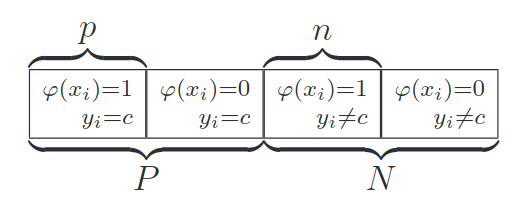
\includegraphics[scale=0.6]{Dissertation/images/DISSER-44.png}
    }
    \caption{О понятии информативности}\label{fig:inform}
\end{figure}

Мера информативности определяется какое количество позитивных объектов он выделяет. Задача построения информативного предиката $\phi$ формулируется посредством следующих задач оптимизации:

\begin{equation}
    \label{eq:equation30}
   p_{c}(\phi) \rightarrow max 
\end{equation}

\begin{equation}
    \label{eq:equation31}
    n_{c}(\phi) \rightarrow min
\end{equation}

Позитивные объекты, выделенные предикатом задаются в виде:

\begin{equation}
    \label{eq:equation32}
    D_{c}(\phi, X^{l}) = \frac{p_{c}(\phi)}{l}
\end{equation}

Негативные объекты, выделенные предикатом задаются в виде:

\begin{equation}
    \label{eq:equation33}
    E_{c}(\phi, X^{l}) = \frac{n_{c}(\phi)}{p_{c}(\phi) + n_{c}(\phi)}
\end{equation}

Предикат \phi(x) называется логической $\epsilon, \delta$ - закономерностью для класса $c \in Y $, если $E_{c}(\phi, X^{l}) \leq \epsilon $ и 
$D_{c}(\phi, X^{l}) \geq \delta $ при заданном достаточно малом \epsilon и достаточно большом \delta из отрезка $[0,1]$.

Если $n_{c}(\phi) = 0$, то закономерность \phi называется чистой или непротиворечивой. Если $n_{c}(\phi) > 0$, то закономерность \phi называется частичной.

Информативность предиката \phi(x) относительно класса $c \in Y$ по выборке $ X^{l}$:

\begin{equation}
    \label{eq:equation34}
    I_{c}(\phi, X^{l}) = -ln h \Bigg(
    \begin{matrix}
    p_{c}(\phi) & n_{c}(\phi) \\
    P_{c} & N_{c}
    \end{matrix}
    \Bigg)
\end{equation}

При этом следует учесть, что $ I_{c} \equiv I_{c}(\phi) \equiv I_{c}(\phi, X^{l}) $.

Сформулируем статистическое определение информативности посредством техники проверки статистических гипотез. Пусть $X$ - вероятностное пространство , выборка $X^{l}$ - простая, то есть случайная, независимая, одинаково распределенная, $y^{*}(x), \phi(x)$ - случайные величины.
 Допустим, что гипотеза о независимости событий справедлива:

\begin{equation}
    \label{eq:equation35}
    \{x: y^*(x) = c\} , \{x: \phi(x) = 1\}
\end{equation}

Тогда вероятность реализации пары $(p, n)$ возможно выразить через следующее гиперпараметрическое распределение:

\begin{equation}
    \label{eq:equation36}
    \left h\Bigg( 
    \begin{matrix}
    p & n \\
    P & N
    \end{matrix}
     \Bigg)
    =
    \frac{C_P^p C_N^n}{C^{p+n}_{P+N}}, 0 \leq p \leq P, 0 \leq n \leq N \right
\end{equation}

где

\begin{equation}
    \label{eq:equation37}
    C^{k}_m = \frac{m!}{k!(m-k)!}, 0 \leq k \leq m.
\end{equation}

Таким образом, если событие с малой вероятностью реализовалось, то, скорее всего, оно не случайно. Неслучайное событие это и есть закономерность.

Определим информативность предиката \phi(x) относительно класса $c \in Y $ по выборке $X^{l}$:

\begin{equation}
    \label{eq:equation38}
    I_c(\phi, X^{l}) = - ln h \Bigg(
    \begin{matrix}
    p_c(\phi) & n_c(\phi) \\
    P_c & N_c
    \end{matrix}
    \Bigg)
\end{equation}

Предикат \phi(x) будем называть статистической закономерностью для класса $c$ в случае, если при заданном достаточно большом $I_0$ справедливо следующее неравенство:

\begin{equation}
    \label{eq:equation39}
    I_c(\phi, X^{l}) \geq I_0
\end{equation}


Уровень значимости для порога информативности $I_0$ выбирается достаточно малым для проверки статистических гипотез о независимости событий.

Для вычисления информативности воспользуемся приближенным методом расчета Стирлинга:
\begin{equation}
    \label{eq:equation40}
    ln k! \approx \Bigg( k + \frac{1}{2} \Bigg) ln k - k + \frac{1}{2}ln2\pi + \frac{1}{12k} - \frac{1}{360k^2}
\end{equation}

Существует два исхода $\omega_{0}, \omega_{1}$ с вероятностями $q_{0}$ и $q_{1} = 1 - q_{0}$. Количество информации, связанное с исходом $\omega_{i}$ равно $-log_{2}(q_{i})$.

Энтропия определяется, как математическое ожидание от количества информации:

\begin{equation}
    \label{eq:equation41}
    H(q_0, q_1) = - q_{0}log_{2}q_{0} - q_{1}log_{2}q_{1}
\end{equation}

Появление объекта класса $c$ с исходом $\omega_0$, а появление любого другого класса $\omega_1$. Энтропия выборки X^{l} вычисляется на основе оценки вероятности исходов, как частоты:

\begin{equation}
    \label{eq:equation42}
    \widehat{H}(P,N) = H \Bigg(\frac{P}{P+N}, \frac{N}{P+N} \Bigg)
\end{equation}

Таким образом, после получения информации $\phi$ энтропия всей выборки становится равной:

\begin{equation}
    \label{eq:equation43}
    \left \widehat{H}(P,N,p,n) = \frac{p+n}{P+N}\widehat{H}(p,n) + \frac{P+N-p-n}{P+N}\widehat{H}(P-p, N-n)\right
\end{equation}

Уменьшение энтропии принимет вид и называется информационным выигрышем:

\begin{equation}
    \label{eq:equation44}
    IGain_{c}(\phi, X^{l}) = \widehat{H}(P,N) - \widehat{H}_{\phi}(P,N,p,n)
\end{equation}

Предикат \phi является закономерностью по энтропийному критерию информативности, если $IGain_{c}(\phi, X^{l}) > G_{0}$ при некотором достаточно большом $G_{0}$. Энтропийный критерий асимптотически эквивалентен статистическому:

\begin{equation}
    \label{eq:equation45}
    IGain_{c}(\phi, X^{l}) \rightarrow \frac{1}{l ln 2}I_{c}(\phi, X^{l}), при l \rightarrow \infty
\end{equation}

Статистический критерий информативности на случай произвольного числа классов $Y = {1,...,M}$:

\begin{equation}
    \label{eq:equation46}
    \left I(\phi, X^{l}) = -ln\frac{C^{p_{1}}_{P_{1}} ... C^{p_{M}}_{P_{M}}}{C^{p}_{l}}\right
\end{equation}

где $P_{c}$ - число объектов класса $c$ в выборке $X^{l}$, из них $p_{c}$ объектов выделяются предикатом $\phi, p = p_1 + p_2 + p_3 + ... + p_M$.

Энтропийный критерий для произвольного числа классов принимает вид и имеет асимптотическое приближение к статистическому:

\begin{equation}
    \label{eq:equation47}
    \left I(\phi, X^{l}) = \sum_{c \in Y} h \Bigg(\frac{P_c}{l} - \frac{p}{l}\sum_{c \in Y}h \Bigg( \frac{p_{c}}{p} \Bigg) - 
    \frac{l-p}{l}\sum_{c \in Y} h \Bigg(\frac{P_c - p_c}{l - p}\Bigg)\Bigg)  \right
\end{equation}

где $h(z) \equiv - z log_{2} z$.

Для выявления закономерностей используется алгоритм бустинга адаптированный для взвешенного голосования. В бустинге строятся последовательные закономерности, после построения очередного вектора весов закономерностей вектор пересчитывается. Веса выделенных для закономерностей объектов изменяются: у позитивных уменьшаются, у негативных увеличиваются. Обновленный вектор  весов $\omega$ используется при поиске следующей закономерности $\phi$ по критерию максимума взвешенной информативности.
Веса объектов и веса закономерностей на каждом шаге алгоритма изменяеются согласно критерию взвешенной информативности~\cref{eq:subeq_1, eq:subeq_2}.

\begin{subequations}
    \label{eq:subeq_1}
    \begin{gather}
        P_{c}^{\omega} = \sum_{i=1}^{l}\omega_{i}[y_{i} = c]; \label{eq:subeq_1-1} \\
        p_{c}^{\omega}(\phi) = \sum_{i=1}^{l}\omega_{i}[y_{i} = c][\phi(x_{i}) = 1]
    \end{gather}
\end{subequations}

\begin{subequations}
    \label{eq:subeq_2}
    \begin{gather}
       N_{c}^{\omega} = \sum_{i=1}^{l}\omega_{i}[y_{i} = c]; \label{eq:subeq_2-1} \\
       n_{c}^{\omega}(\phi) \neq \sum_{i=1}^{l}\omega_{i}[y_{i} = c][\phi(x_{i}) = 1]
    \end{gather}
\end{subequations}


где $\omega$ веса объектов $\omega = (\omega_i)^{l}_{i=1}$,

условие нормировки имеет вид $\sum^{l}_{i=1}\omega_{i} = l$ ,

$P^{\omega}_c$ - число объектов класса $c$ в выборке $X^{l}$,

$p^{\omega}_c$ - из них число объектов, для которых выполняется условие $\phi(x) = 1$,

$N_{c}^{\omega}$ - число объектов всех остальных классов $Y  {c}$ в выборке $X^{l}$,

$n_c^{\omega}(\phi)$ - из них число объектов, для которых выполняется условие $\phi(x) = 1$.

Гипергеометрическое распределение будет вычисляться по следующей формуле:

\begin{equation}
    \label{eq:equation48}
    ln \(z\)! \approx ([z+1] - z)ln[z]! + (z - [z])ln[z+1]!, z \in \mathbb{R}
\end{equation}

\subsection{Модель Библиотекаря для классификации}\label{sec:ch2/sec4/sub4}


Цель - разработать модель в соответствии с вышеописанными принципами:
для этого необходимо входным переменным $X = {x_1, x_2, ..., x_n}$ поставить в соответствие выходные $Y = {y_1, y_2, ..., y_n}$. Первым необходимоым принципом является преобразование базы знаний. Данная операция изображена на Рисунке ~\cref{fig:NNprin}.
\begin{figure}[ht]
    \centerfloat{
        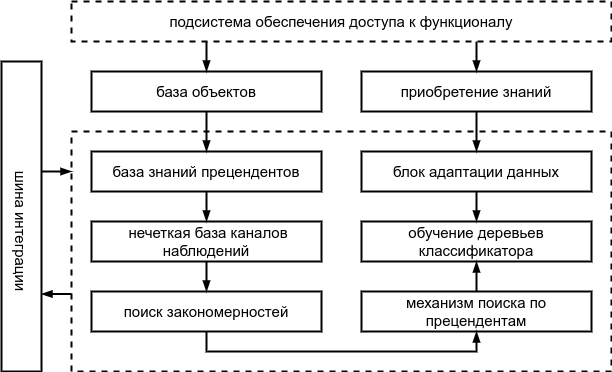
\includegraphics[scale=0.8]{Dissertation/images/DISSER-56.png}
    }
    \caption{Структура принципа преобразования}\label{fig:NNprin}
\end{figure}

Модель классификатора состоит из следующих алгоритмических блоков и называется "моделью Библиотекаря" так как основным ядром классификации является критерий максимума информативности:

\begin{enumerate}
	\item генерация обучающих выборок из каналов наблюдения таблицы ТРИЗ с помощью алгоритма бутстрепа, изображенного на Рисунке ~\cref{fig:bootstrap},
	\item вычисление списков закономерностей с выявлением значения весовых функций для каждого класса из обучающей выборки с помощью алгоритма бустинга,
	\item синтез решающего дерева на основе списков закономерностей для каждого класса,
	\item классификация параметров или каналов наблюдения по критерию максимума информативности,
	\item составление ансамбля деревьев для голосования согласно принципу максимума взвешенной информативности.
\end{enumerate}


\begin{figure}[ht]
    \centerfloat{
        
\includegraphics[scale=1.0]{Dissertation/images/DISSER-46.png}
    }
    \caption{генерация обучающих выборок с помощью алгоритма бутстрепа}\label{fig:bootstrap}
\end{figure}

Алгоритм бутстрепа позволяет выявить списки закономерностей на основе построения выпуклой комбинации закономерностей. Этот алгоритм последовательно строит закономерности, при этом на каждом этапе построения весовые коэффициенты закономерностей обновляются согласно критерию максимума взвешенной информативности. 

Для проведения обучения на обучающей выборке в модели используется алгоритм бустинга. Для определения закономерности, которая совершает минимальное количество ошибок на обучающей выборке $X^{l}$  распишем функционал числа ошибок алгоритма $a_{T+1}(x)$, с помощью тождества 
$e^{A\phi} = (1-\phi)+\phi e^{A}, A \in \textbb{R}, \phi \in {0,1} $:

\begin{equation}
    \label{eq:equation51}
     \begin{multlined}
    \tilda{Q}_{T+1} = \sum_{i=1}^{l}\omega_{i}e^{-\alpha\phi_c(x_i)}[y_{i} = c] + \sum_{i=1}^{l}\omega_{i}e^{\alpha\phi_c(x_i)[y_i \neq c]} = \\
    = \sum_{i=1}^{l}\omega_{i}(1-\phi_c(x_i)) + e^{-\alpha}\sum_{i=1}^{l} \omega_{i} \phi_c(x_i) [y_{i} = c] +
    \\
    + e^{\alpha}\sum_{i=1}^{l}\omega_{i}\phi_{c}(x_i)[y_i \neq c]
     \end{multlined}
\end{equation}

Выразим минимум этого функционала , который достигается при $e^{-\alpha}p = e^{\alpha}n$, $\alpha^* = \frac{1}{2}ln\frac{p}{n}$:
\begin{equation}
    \label{eq:equation52}
    \begin{multlined}
    \tilda{Q}_{T+1} = \frac{\tilda{Q}_{T}}{l} \Bigg( \sum_{i=1}^{l}\tilda{\omega}_{i} - \sum_{i=1}^{l}\tilda{\omega}_{i}\phi_{c}(x_{i}) +
    \\
    +
    e^{-\alpha}\sum_{i:y_{i}=c}\tilda{\omega}_{i}\phi_{c}(x_{i}) + e^{\alpha}\sum_{i:y_{i} \neq c}\sum_{i:y_{i} \neq c}\tilda{\omega}_{i}\phi_{c}(x_i)  \Bigg) = \\
    = \frac{\tilda{Q}_{T}}{l} (l - p^{w}_{c}(\phi_c) - n^{\omega}_c(\phi_c) + e^{-\alpha}p^{w}_{c}(\phi_c) +e^{\alpha}n^{\omega}_c(\phi_c))
    \end{multlined}
\end{equation}

Минимум достигается при $e^{-\alpha}p^{w}_{c}(\phi_c) = e^{\alpha}n^{\omega}_c(\phi_c)$, где $\alpha^* = \frac{1}{2}ln{\frac{p}{n}}, n \neq 0$:
\begin{equation}
    \label{eq:equation53}
    \begin{multlined}
    \tilda{Q}_{T+1} = \frac{\tilda{Q}_T}{l} \Bigg( l - p^{w}_{c}(\phi_c) - n^{\omega}_c(\phi_c) + 
    \\
    + p^{w}_{c}(\phi_c)\sqrt{\frac{ n^{\omega}_c(\phi_c)}{p^{w}_{c}(\phi_c)}} + n^{\omega}_c(\phi_c) \sqrt{\frac{p^{w}_{c}(\phi_c)}{ n^{\omega}_c(\phi_c)}}\Bigg) =
    \\
    = \tilda{Q}_{T}\Bigg( 1 - \frac{1}{l} (\sqrt{p^{w}_{c}(\phi_c)} - \sqrt{n^{\omega}_c(\phi_c)})^{2} \Bigg)
    \end{multlined}
\end{equation}

Для того, чтобы избежать неограниченного убывания функционала $\tilda{Q}_{T+1}$ при $n = 0$, введем дополнительный параметр $\lambda \in {0,1}$ для расчета формулы весов:
\begin{equation}
    \label{eq:equation54}
    \alpha^* = \frac{1}{2}ln\frac{{p^{w}_{c}(\phi^{*}_{c})}}{max \{n^{\omega}_c(\phi^*_c), \lambda\}}
\end{equation}

Таким образом, закономерность \phi определяется как:
\begin{equation}
    \label{eq:equation55}
    J^{\omega_c}_c(\phi_c) = \sqrt{p^{w}_{c}(\phi_c)} - \sqrt{n^{\omega}_c(\phi_c)}
\end{equation}

Веса закономерностей пересчитываются следующим образом:
\begin{equation}
    \label{eq:equation56}
    {\omega'}_{i} = \omega_i\Bigg( [y_i = c] e^{−\alpha\phi_c(x_i)} 
    + [y_i \neq c] e^{\alpha\phi_c(x_i)}] \Bigg) 
\end{equation}


\begin{equation}
    \label{eq:equation57}
\[ {\omega'}_{i} = \begin{cases}
    \omega_{i},       & \phi_c(x_i) = 0; \\
    \omega_{i}e^{-\alpha},       & \phi_c(x_i) = 1, y_i = c; \\
    \omega_{i}e^{\alpha},       & \phi_c(x_i) = 1, y_i \neq c; 
  \end{cases}
\]
\end{equation}


Принцип голосования основывается на подсчете голосов следующим образом, указанным на Рисунке ~\cref{fig:voting}. Пусть множество правил $ R_{c}$ или логических закономерностей для каждого класса $c \in Y$ будет описано в соответствии со следующей формулой:

\begin{equation}
    \label{eq:equation49}
    R_{c} = {\phi_{c}^{t}: X \rightarrow {0,1} | t = 1, ..., T_{c}}
\end{equation}

\begin{figure}[ht]
    \centerfloat{
        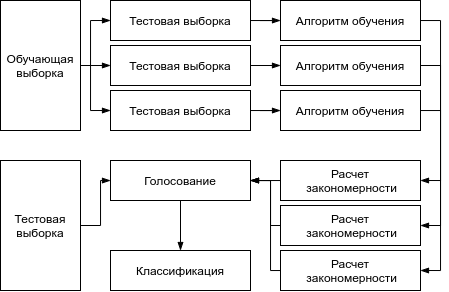
\includegraphics[scale=1.0]{Dissertation/images/DISSER-47.png}
    }
    \caption{Принцип голосования }\label{fig:voting}
\end{figure}

Тогда, если $\phi^{t}_{c} = 1 $, то это значит, что правило $\phi^{t}_{c}$ относит объект $x \in X$ к классу $c$. Если $\phi^{t}_{c} = 1 $, то классификации не происходит.

Голосование присходит следующим образом: каждому правилу $\phi^{t}_{c}$ приписывается вес $\alpha_{c}^{t} \geq 0$ и расчитывается взвешенная сумма голосов:

\begin{equation}
    \label{eq:equation50}
    \Gamma_c(x) = \displaystyle\sum_{t=1}^{T_c} \alpha_c^t\phi_c^t(x), \alpha_c^t \geq 0
\end{equation}

Веса нормируются до единицы $\displaystyle\sum_{t=1}^{T_c}\alpha_c^t = 1$ для всех $c \in Y$. Таким образом фнукция подсчета взвешенного голосования образует выпуклую комбинацию правил  $\phi_c^1 ,  ... , \phi_c^t$.

\subsection{Требования к модели}\label{sec:ch2/sec3/sub5}
Проектирование архитектуры автоматизированной системы является наиболее абстрактным и наиболее идеализированным представлением системы, которое должно обеспечивать выполнение следующих свойств:
\begin{enumerate}
\item элементы архитектуры должны быть слабо связаны таким образом, чтобы разложив на декомпозицию элементов, поток информации, проходящий по контурам был минимальным и не замыкался;
\item должно соблюдаться свойство тестируемости, т.е. при проверки работы функций системы должен быть установлен факт правильной работы;
\item должна соблюдаться возможность идентификации неисправных частей системы путем диагностики;
\item должно соблюдаться свойства восстановления системы в кратчайшие сроки с экономически обоснованной стоимостью ремонта;
\item должно соблюдаться свойство надежности;
\item система должна быть проста в обслуживании и проста в эксплуатации, не требовать высокой квалификации и повышения квалификации обслуживающего персонала;
\item система и ее составляющие элементы должны быть безопасны в эксплуатации, должны соблюдать требования охраны труда и техники безопасности;
\item система должны быть обеспечена защитой от вандализма и неавторизованных пользователей;
\item система должна проектироваться с учетом эффективности в отношении затрачиваемых ресурсов в  операционном процессе;
\item система должна уметь выстаиваивать новые конфигурации, создавать новые настройки для работы с другими технологическими процессами;
\item система должна уметь функционально расширяться, т.е. в логика работы должна уметь дополняться дополнительными функциональными возможностями системы;
\item система должны быть готова к устойчивому масштабированию системы, таким образом, чтобы увеличение размера объекта автоматизации не требовало высоких затрат и не сводила к неустойчивому состоянию базовую модель системы;
\item система должна быть открытой, таким образом, чтобы можно было заменить один модуль системы на аналогичный модуль другого производителя, а интеграция модулей происходила без чрезмерных конфликтов и проблем;
\item система должна стремиться к максимально продолжительному жизненному циклу без значительного устаревания, который должен обновлять аппаратные и программные компоненты;
\item система должна устанавливаться и вводиться в эксплуатацию за минимальное время.
\end{enumerate}

Таким образом, модель должна соблюдать перечисленные выше технические требования.

Принцип реализации сводится к адаптации информации, сформированной на базе фактов с пользовательским запросом на обработку и выдачу рекомендаций по проектированию. Общая схема движения информационного потока представлена на Рисунке~\cref{fig:Dataflow} 

\begin{figure}[ht]
    \centerfloat{
        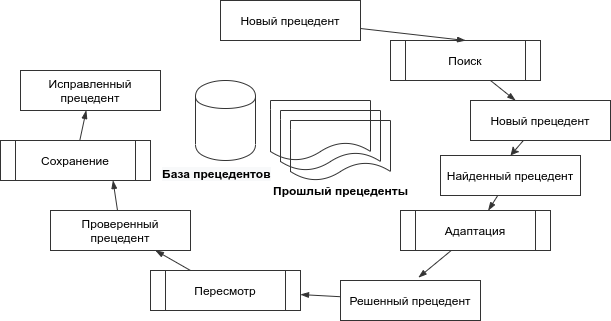
\includegraphics[scale=0.8]{Dissertation/images/DISSER-16.png}
    }
    \caption{Структура принципа преобразования}\label{fig:Dataflow}
\end{figure}
Для построения модели накладываются следующие ограничения:
\begin{enumerate}
	\item критерий максимума взвешенной информативности, позволяющий определить предикаты, как закономерности~\cref{eq:subeq_1, eq:subeq_2},
	\item критерий поиска конъюктивных закономерностей для отбора признаков ~\cref{eq:equation55, eq:equation56},
	\item мера информативной энтропии ~\cref{eq:equation47},
	\item экспоненциальная аппроксимация пороговой функции потерь ~\cref{eq:equation54}.
\end{enumerate}

Требования для разработки системы поддержки принятия решений вырабатываются на основе анализа проблем в области задачи принятия решений. Например, для поддержки принятия решений в области проектирования программного обеспечения крайне сложно анализировать организацию шаблонов проектрования кода на уровне отношений между сущности, также довольно сложнореализуемой задачей является анализ индексации таблиц и определения внешний и составных ключей, отношений между таблицами в БД.

Таким образом, основными требованиями при разработке модели поддержки принятия решений выступили требования по формированию вектора рекомендаций для проектирования того или иного набора инструментов для реализации задач проектирования. Для решения такой задач, после проведения анализа проблематики и выявления альтернатив, была разработана модель классификации на основетаблицы ТРИЗ, где каналы наблюдения выражены посредством инструмента нечеткой логики. Требования к модели принятия решений блоком классификатора, главным образом, определялся возможностью реализации конъюнкционного вывода на основе поиска закономерностей, но с возможностью обновления и адаптации под пользовательские запросы. Система должна уметь адаптироваться под запросы пользователей, а также адаптировать свою семантическую структуру закономерностей дополняя базу новыми наблюдениями, новыми прецендентами.

Основные требования при проектирования модели поддержки принятия решений перечислены здесь:

\begin{enumerate}
	\item система должна уметь интерпретировать слабоструктурированный текст в семантически верную закономерность,
	\item система должна уметь выявлять эвристические закономерности и аппроксимировать функционал оптимизации подбора рекомендаций,
	\item система должна уметь выявлять закономерности,
	\item система должна уметь обрабатывать отношения между объектами,
	\item система должна уметь формировать рекомендацию.
\end{enumerate}


\subsection{Алгоритмическое описание модели}\label{sec:ch2/sec4/sub2}

Цель - разработать алгоритм в соответствии с вышеописанными принципами:
для этого необходимо входным переменным $X = {x_1, x_2, ..., x_n}$ поставить в соответствие выходные $Y = {y_1, y_2, ..., y_n}$. Первым необходимоым принципом является преобразование базы знаний. Данная операция изображена на Рисунке ~\cref{fig:NNprin}.
\begin{figure}[ht]
    \centerfloat{
        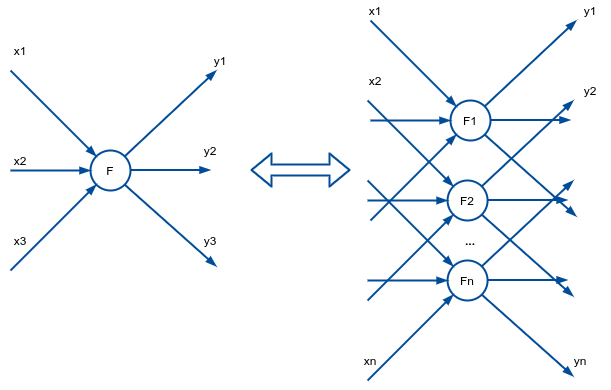
\includegraphics[scale=0.5]{Dissertation/images/DISSER-18.png}
    }
    \caption{Структура принципа преобразования}\label{fig:NNprin}
\end{figure}

Обобщенный алгоритм классификатора приведен на Рисунке~\cref{fig:commonclassificator}

\begin{figure}[ht]
    \centerfloat{
        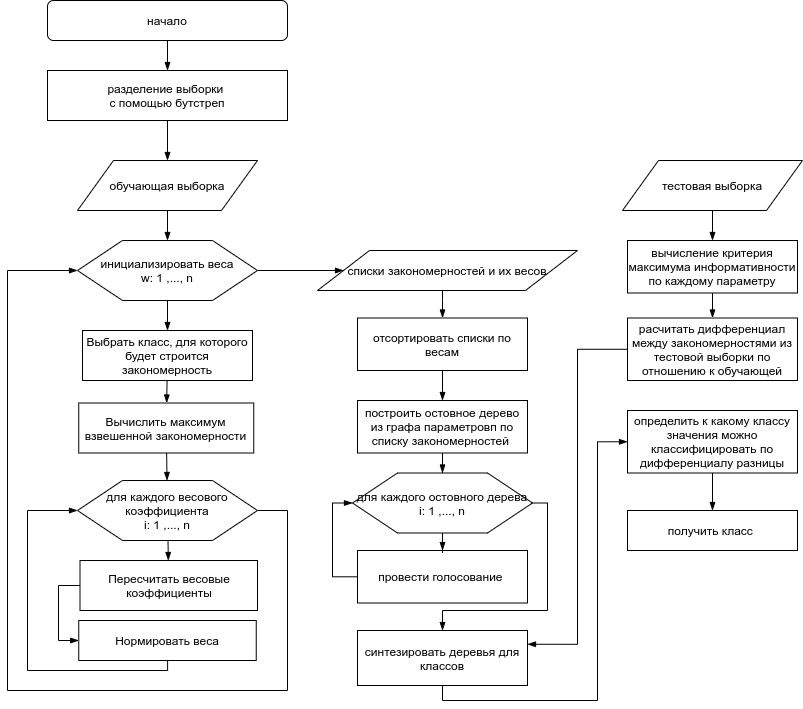
\includegraphics[scale=0.6]{Dissertation/images/DISSER-49.png}
    }
    \caption{Обобщенный алгоритм классификатора }\label{fig:commonclassificator}
\end{figure}


\begingroup
\centering
\small
\captionsetup[table]{skip=7pt} % смещение положения подписи
\begin{longtable}[c]{|l|c|l|l|}
    \caption{Алгоритмическое описание модели}\label{tab:test5}% label всегда желательно идти после caption
    \\[-0.45\onelineskip]
    \hline
    Шаг & Знач. по ум.& Тип & Описание                                          \\ \hline
    \endfirsthead%
    \caption*{Продолжение таблицы~\thetable}                                    \\[-0.45\onelineskip]
    \hline
    Шаг & Знач. по ум. & Тип & Описание                                          \\ \hline
    \endhead
    \hline
    \endfoot
    \hline
    \endlastfoot
    \multicolumn{4}{|l|}{\&INP}                                                 \\ \hline
    Входные     &       & double & 0: инициализация без шума (\(p_s = const\))\\
    данные         &        &     & 1: генерация и случайный отбор данных \\
             &        &     & из общих наблюдений \\
             &        &     & 2: применение операции случайного выбора \\
             &        &     & выборки из совокупности \\
             &        &     & 3: процедура перевыбора выборкив в цикле         \\
             &        &     & 4: вычисление среднего в цикле       \\
             &        &     & по каждой выборке                         \\
             &        &     & 2: генерация белого шума симметрично относительно \\
             &        &     & экватора                                          \\
    Поиск    & rand   & double & 0: инициализация весов случайными значениями   \\
    законо-  &        &     & или по оценкам       \\
    мернос-  &        &     & 1: выбор класса для построения закономерности    \\
    тей      &        &     & в цикле \\
    в обу-   &        &     & 2: внутри каждого выбранного класса рассчитать \\
    чающей   &        &     & $\phi^t_c = argmax_{\phi \in \Phi}\sqrt{\phi^w_c(\phi) - \sqrt{n^w_c(\phi)}}$\\
    выборке  &        &     & 4: внутри каждого выбранного класса рассчитать \\
             &        &     & $\alpha^t_c = \frac{1}{2}ln\frac{{p^{w}_{c}(\phi^{*}_{c})}}{max \{n^{\omega}_c(\phi^*_c), \lambda\}}$\\
             &        &     & 5: для всех $i = 1,...,l $  пересчитать вес \omega_i$ \\
             &        &     & 6: для всех $i = 1,...,l $  нормировать вес \omega_i$ \\
    Голо-    &        &double& 1: для всех $i = 1,...,l $  деревьев   \\
    вание    &        &     & 2: для каждой закономерности $\phi^{t}_{c}$ \\
             &        &     & приписывается вес $\alpha_{c}^{t} \geq 0$  \\
             &        &     & 3: расчитывается взвешенная сумма голосов         \\
             &        &     & $ \Gamma_c(x) = \displaystyle\sum_{t=1}^{T_c} \alpha_c^t\phi_c^t(x), \alpha_c^t \geq 0$\\
\end{longtable}
\normalsize% возвращаем шрифт к нормальному
\endgroup

Алгоритм бутстрепа состоит из следующих шагов и изображен на Рисунке ~\cref{fig:bootstrap}:
\begin{enumerate}
	\item формируется случайная выборка на основе генеральной совокупности из общего числа наблюдений,
	\item к каждой отобранной выборке применяется случайная операция выбора с возвратом того же размера,
	\item процедура перевыбора применяется многократное количество раз и выбирается среднее,
	\item из вычисленных средних по всем наборам вычислить среднее и рассматривать как среднее из генеральной совокупности.
\end{enumerate}

Алгоритм построения бустинга состоит из следующих шагов, изображенных на Рисунке  ~\cref{fig:busting}:
\begin{enumerate}
	\item на вход подается $X^l$ обучающая выборка, $\Phi$ семейство базовых предикатов, $T$ семейство базовых предикатов, $\lambda$ - коэффициеннт поощрения непротиворечивых закономерностей,
	\item на втором шаге инициализируются веса $\omega_i : = 1 $  для всех $i = 1, 2, ... , l$,
	\item далее для всех $t = 1, ... , T$ выбрать класс, для которого строится закономерность $c: c_t$:
	\begin{enumerate}
		\item внутри каждого выбранного класса рассчитать $\phi^t_c = argmax_{\phi \in \Phi}\sqrt{\phi^w_c(\phi) - \sqrt{n^w_c(\phi)}}$,
		\item внутри каждого выбранного класса рассчитать $\alpha^t_c = \frac{1}{2}ln\frac{{p^{w}_{c}(\phi^{*}_{c})}}{max \{n^{\omega}_c(\phi^*_c), \lambda\}}$,
		\begin{itemize}
			\item для всех $i = 1,...,l $  пересчитать вес \omega_i$,
			\item нормировать веса.
		\end{itemize}
	\end{enumerate}
\end{enumerate}

\begin{figure}[ht]
    \centerfloat{
        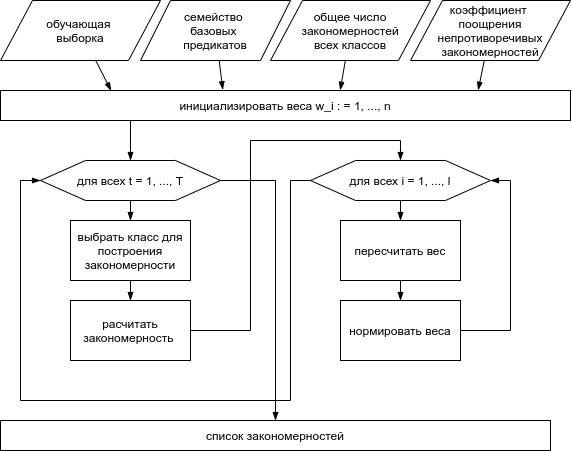
\includegraphics[scale=0.7]{Dissertation/images/DISSER-50.png}
    }
    \caption{Алгоритм построения бустинга }\label{fig:busting}
\end{figure}

Алгоритм голосования состоит из следующих шагов:
\begin{enumerate}
	\item для каждого дерева $i = 1, ..., n$:
	\begin{enumerate}
		\item для каждой закономерности $\phi^{t}_{c}$ приписывается вес $\alpha_{c}^{t} \geq 0$,
		\item расчитывается взвешенная сумма голосов $ \Gamma_c(x) = \displaystyle\sum_{t=1}^{T_c} \alpha_c^t\phi_c^t(x), \alpha_c^t \geq 0$.
	\end{enumerate}
\end{enumerate}

 Общая идея алгоритма голосования изображена на Рисунке ~\cref{fig:votesum}
\begin{figure}[ht]
    \centerfloat{
        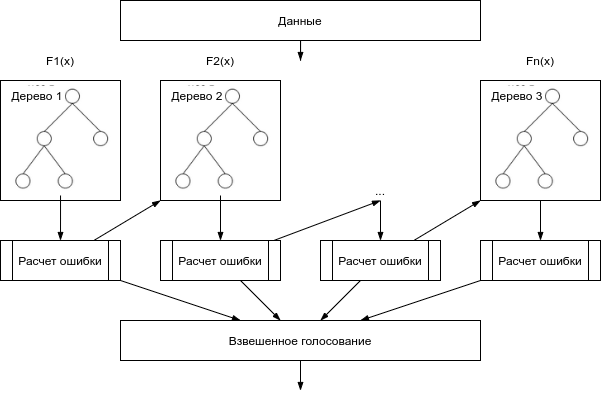
\includegraphics[scale=0.7]{Dissertation/images/DISSER-48.png}
    }
    \caption{Алгоритм построения бустинга }\label{fig:votesum}
\end{figure}


\subsection{Модель информационного обмена при проектировании системы поддержки принятия решения}\label{sec:ch2/sec3/sub3}
На рисунке ~\cref{fig:NNmodel} представлена работа блоков деревьев обработчиков классификатора. Все блоки взаимосвязанны друг с другом и образуют интеллектуальную модель поддержки принятия решений.
\begin{figure}[ht]
    \centerfloat{
        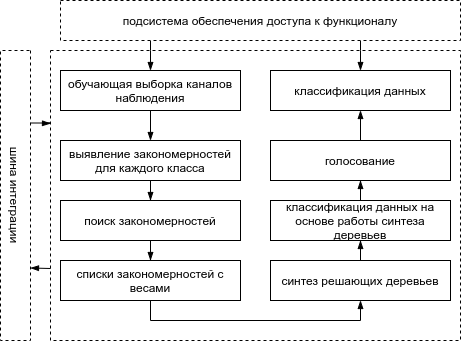
\includegraphics[scale = 0.8]{Dissertation/images/DISSER-1.png}
    }
    \caption{Работа блоков деревьев обработчиков классификатора}\label{fig:NNmodel}
\end{figure}

Основные блоки интеллектуального модуля поддержки принятия решений это:

\begin{enumerate}
    \item база объектов, описывающая параметры конфигурации типовых информационных систем,
    \item база знаний прецендентов, сформированная базой объектов,
    \item нечеткая база знаний из каналов наблюдений, формируемая на основе закономерностей, получаемых из обучающей выборки,
    \item нейронечеткий механизм, который обучается и формирует нечеткую функцию рекомендаций,
    \item блок адаптации данных, данный блок принимает на вход данные получаемые от пользовательских запросов к системе,
    \item блок обучения деревьев классификатора, где происходит обучение механизма выявления закономерностей,
    \item механизм поиска по прецендентам, где происходит обработка запросов и сопостовление процедента с предъявляемым параметром или каналом наблюдения.
\end{enumerate}

На рисунке ~\cref{fig:NNproc} представлена модель обработки данных в укрупненном масштабе. 
\begin{figure}[ht]
    \centerfloat{
        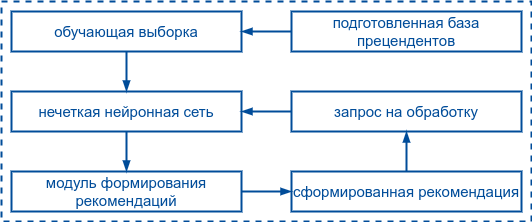
\includegraphics[scale=0.8]{Dissertation/images/DISSER-2.png}
    }
    \caption{Модель обработки данных }\label{fig:NNproc}
\end{figure}

Если рассматривать задачу с точки зрения теории управления, то мы получаем адаптивную комбинированную систему автоматизированного управления (т.к. обучение происходит с участием человека) с возмущением. 
Управляющая система представлена на рисунке ~\cref{fig:NNsau} в укрупненной абстракции. 
\begin{figure}[ht]
    \centerfloat{
        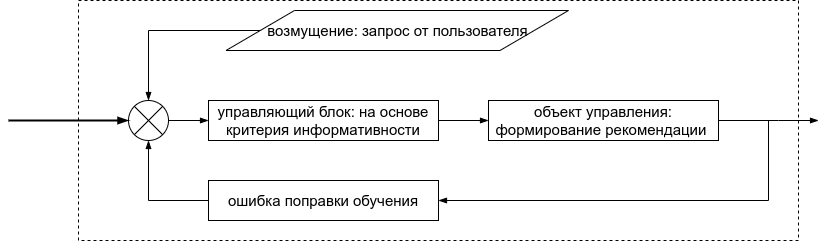
\includegraphics[scale=0.65]{Dissertation/images/DISSER-3.png}
    }
    \caption{Модель обработки данных }\label{fig:NNsau}
\end{figure}

Сравнительная таблица методов управления представлена на Рисунке ~\cref{fig:Csau}
\begin{figure}[ht]
    \centerfloat{
        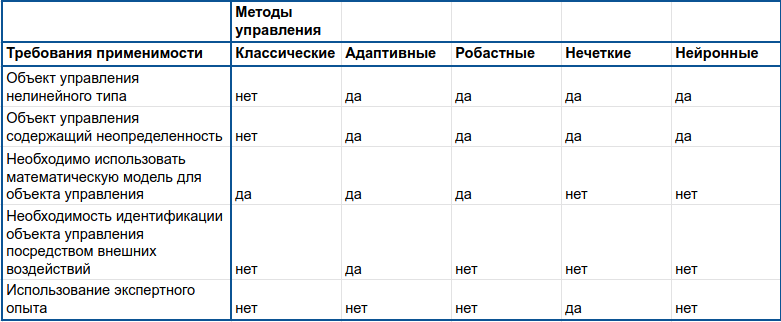
\includegraphics[scale=0.65]{Dissertation/images/DISSER-19.png}
    }
    \caption{Сравнительная таблица методов управления}\label{fig:Csau}
\end{figure}

Модель поддержки принятия решения может быть рассмотрена, как система автоматического управления с возмущением комбинированного типа. Входная информация поступает на линейный вход в модель обаботки информации и структуризации семантических данных ${z}$, обратная связь послупает от модуля расчета ошибки работы нейронной сети, здесь к управляющей системе возвращается информация о состоянии объекта управления ${у}$. Информация о состоянии объекта управления и возмущении ${w}$ поступает на вход к объекту управления, далее информация обрабатывается в соответствии с целью формирования рекомендаций, где объект управления получает воздействия от блока управления в виде набора рекомендаций и в виде управляющих воздействий передается на объект управления
\begin{equation}
    \label{eq:equation30}
    S = \{S_y, O_y, C,  \overrightarrow{z}, \overrightarrow{y}, \overrightarrow{w}\}
\end{equation}

Модель вычислений представлена в виде
\begin{equation}
    \label{eq:equation30}
    E_S=<K_B,F_B,R_B,I^e,R^e>
\end{equation}


где $K_B$- база знаний в виде закономерностей; 

$F_B$- таблица фактов $S$;

$R_B$- таблица закономерностей, создаваемая модулем интерпретатором в ходе вычислений, содержит информацию о причинах возникающих изменений в базе правил, а также поправки, комментарии, внесенные экспертом в базу знаний для объяснений; 

$R^e$ — отношения между объектами; 

$I^e$ — интерпретатор, который опирается на последовательное исполнение: $I^e =<I^{e1}, I^{e2}, I^{e3}, I^{e4}>$,

$I^{e1}$ - процесс выбора из базы знаний подмножества необходимых закономерностей; 

$I^{e2}$ - процесс сверки с прецендентами; 

$I^{e3}$ - процесс принятия оптимального решения; 

$I^{e4}$ — процесс отбора по критерию максимума взвешенной информативности.

Модель системы интеллектуального вывода может быть представлена следующим образом
\begin{equation}
    \label{eq:equation31}
    NN=<A_r,X,Y,M^n,E_d,I^{n1}, I^{n2} >,
\end{equation}

где $A_r$ — топология деревьев классификации на класс для принятия решений и вывода рекомендации; 

$X, У$ - множества входов и выходов для модуля обработки деревьев соответственно; 

$М^n$ — множество деревьев классификации; 

$E_d$ — обучающая и тестирующая выборки; 

$I^{n1}, I^{n2}$ — интерпретаторы обучения и вычислений деревьев принятия решений и формулирования рекомендаций.

Таким образом, интегрированная система деревьев  принятия решений для экспертного вывода модели вычислений будет иметь следующий вид
\begin{equation}
    \label{eq:equation32}
    NES=<K_B,X,Y,M^n,E_d,R_e, I^{n1}, I^{n2} >
\end{equation}

В экспертной системе с дереьвями принятия решений сохраняется база закономерностей экспертной системы, с помощью которой строится система экспертного вывода с некоторыми входами $X$ и выходами $Y$, где $E_d$ — обучающая и тестирующая выборки модели поддержки принятия решений;  $I^{n1}, I^{n2}$ — интерпретаторы проектируемые для обучения деревьев классификации, а также для формирования рекомендаций соответственно; новая система получает новый набор отношений между объектами в виде $R_e$.

Разработанная в работе модель экспертной системы с деревьями решений проектируется с целью формировать рекомендации. Для извлечений рекомендаций необходимо ввести данные о проектируемой системе согласно шаблону опроса, затем запустить модуль принятия решений. 
Модель вычислений с использованием методов конъюнкционной логики на основе прецедентов имеет следующий вид:

\begin{equation}
    \label{eq:equation33}
    PS=<K_{B1},K_{B2},A(p), I^p >
\end{equation}

где $K_{B1},K_{B2}$- блок прецедентов и блок знаний о проектированнии архитектуры; 

$А(р)$ — алгоритм, который определяет схожие прецеденты р.

Интерпретатор $І_р$, использующий алгоритм $А(р)$ и модуль $К_{В2}$, который обрабатывает данные, хранящиеся в базе знаний $К_{B2}$. Все это может быть представлена как совокупность процессов
\begin{equation}
    \label{eq:equation34}
    I^p = <I^{p1}, I^{p2}, I^{p3}, I^{p4}>
\end{equation}

где $I^{p1}$ - сохранение, 

$I^{p2}$ - обнаружение, 
$I^{p3}$ - адаптация , 
$I^{p4}$ - пересмотр

Гибкость модели обучения записит от следущих параметров

\begin{equation}
    \label{eq:equation35}
    NES^p=<K_B,X,Y,M^n,E_d,R_n, I^{np}, I^{n2}, I^p >
\end{equation}

Конъюнкционные правила сохраняются в виде $K_{B1}$, также в виде прецедентов $K_{B2}$ ; $R^n$ — отношения между объектами представляются в виде некоторого отношения вложенности или принадлежности (определяется семантическим интерпретатором логики). Поиск решений разбивается на решение получаемое с помощью аппроксимации нечеткой логики и работы по выявления прецендентов на основе работы деревьев поиска закономерностей на основе критерия максимума взвешенной информативности $І^р$ с действием алгоритма $А(р)$ определения похожих прецедентов. Обучение $І^р$ производится на основе данных из прецедентов из ТРИЗ графа, состоящего из каналов наблюдения.


\subsection{Алгоритм оценки устойчивости модели}\label{sec:ch2/sec3/sub4}

Рассмотрим следующую систему. Пусть система поддержки решений будет представлена в виде:
\begin{equation}
    \label{eq:equation46}
     \left\{\begin{array}{ll} 
    \dot{x} = X(x,t) \textrm{,} 
    \\ X(0,t) = 0 \textrm{,} 
     \forall{t} \geq t_0
      & \end{array} \right. \]
\end{equation}

Пусть отклик от обучения будет представлен в виде постоянного возмущения $R(x,t)$
\begin{equation}
    \label{eq:equation47}
    \dot{x} = X(x,t) + R(x,t),
\end{equation}

где $R(0,t) \neq 0$ и момент покоя $x = 0$ не является решением данного уравнения.

Положение системы, согласно \cite{Tau}, будет определено, как устойчивое при постоянно действующих возмущениях, если будет существовать такое малое $\varepsilon$ для которого найдутся такая пара положительных $\delta_0$ и $\delta_1$, что при выполнении неравенства $|R(x,t)| < \delta_1$ при всех $|x|\leq \varepsilon$ и $t \geq t_0$, движение возмущения может быть описано неравенством $|x(x^0, t)| < \varepsilon$ и $t \geq t_0$.
В общем смысле система поддержки решений на основе модуля поиска закономерностей при малых отклонениях обучения на экспоненциальную функцию потерь малы т.е. отклонение положения возмущения от невозмущенного положения малы. Определим меру возмущений, согласно теореме Малкина \cite{Tau}
\begin{equation}
    \label{eq:equation48}
    |grad V(x,t)| = \sqrt{\sum_{i=1}^n{\frac{\partial V}{\partial x_i}}^2} \leq N
\end{equation}

где $N$ - положительная константа.

Тогда, система принятий решений и интеллектуальный модуль должны быть ограничены в отклонениях в возмущениях в виде некоторой константы $N$. Таким образом, переобучение или недобучение системы определяются, как состояния, которые выходят за предел допустимого $N$ отклонений в возмущениях.

Выведем последовательность действий при обработке информации в модуле деревьев обработкии поиска закономерностей на основе нечеткого модуля продукционных правил. Представим перечень шагов:
\begin{enumerate}
    \item ввод данных в систему, система получает набор переменных, которые принимают конкретные значения в зависимости от значений введенных данных, данные передаются на вход, множество введенных данных обозначим как $P =\{p_1, p_2, ..., p_n\}$,
    \item сохраняем набор параметров в сущность, создаем сущность описание прецендента,
    \item определяем важности параметров, присваиваем весовые коэффициенты каждому параметру $W = \{W_1, W_2, ..., W_n\}$
    \item сохраняем размерность количества признаков, введеных в систему,
    \item переводим значения характеристик в числовые переменные посредством фукционалов принадлежности,
    \item передаем на обработку в дерево для поиска по таблице фактов,
    \item создаем сущность для агрегированная и обработка промежуточной информации, 
    \item проходим в цикле по всем закономерностям и сохраняем найденное в агрегированную сущность,
    \item в случае отсутствия данных создаем отдельную подсущность для хранения пустых множеств значений параметров переменных отображения, созданная подсущность будет помогать основному каналу наблюдения аппроксимировать данные черех обработку обратного обучения через деревья связи,
    \item в сущносте с отобранными по рангам соответствия всем значениям, проверяем на метрическую принадежность векторов признаков к вектору введенных переменных, используется критерий максимума взвешенной информативности, где прецедент, находящийся в обработке $A_j$ сравнивается с описанным вектором перенесенных запросом $P$, сравнения проходят согласно векторам весов важности в упорядоченном множестве,
    \item производим расчет максимума взвешенной информативности, 
    \item рассчитываем расстояния максимума взвешенной информативности для граничных объектов,
    \item расчитываем шаги сходства, степени возможного правдоподобия или близости $S(A,P) = \frac{(1-D)}{D_{max}}$, нормируем и приводим в долевое выражение от $\{0, ..., 1\}$,
    \item в случае, если не находятся похожие прецеденты , передаем запрос на уменьшение уровня правдоподобия и производим расчеты заново,
    \item в случае заполнения значений и отбору прецедентов не по всем переменным, сохраняем то состояние, что есть и выводим ответ,
    \item сформированный ответ сохраняем в конъюнкционную базу прецедентов для последующего использование.
\end{enumerate}

На Рисунке~\cref{fig:NN1} указано исполнения вышеописанных шагов 1-9, на Рисунке~\cref{fig:NN2} все остальные.
\begin{figure}[ht]
    \centerfloat{
        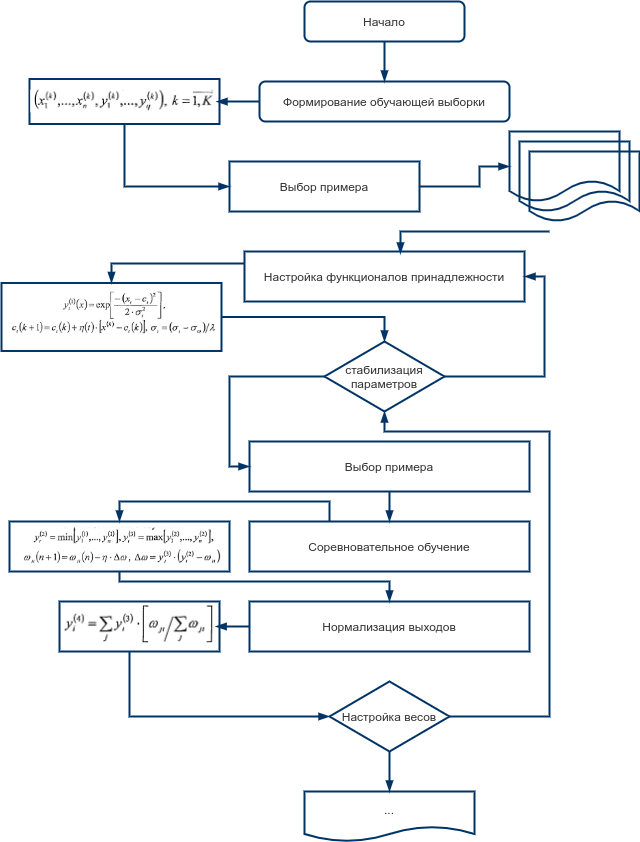
\includegraphics[scale=0.8]{Dissertation/images/DISSER-29.png}
    }
    \caption{Последовательность обработки данных в модуле обработки деревьями поиска закономерностей}\label{fig:NN1}
\end{figure}
\begin{figure}[ht]
    \centerfloat{
        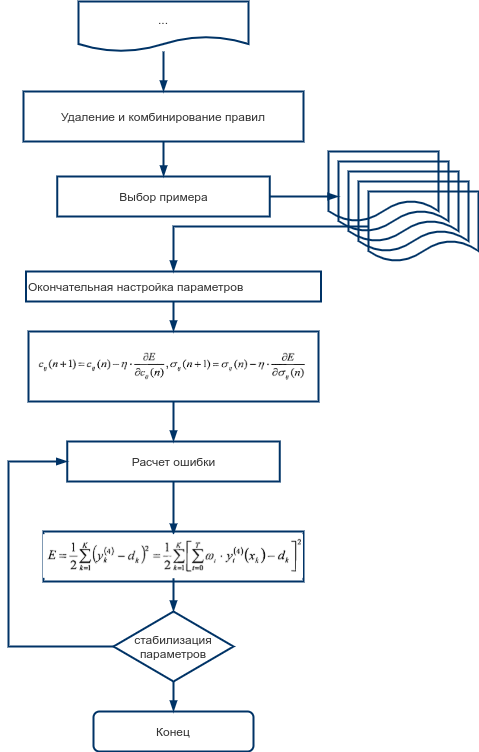
\includegraphics[scale=0.5]{Dissertation/images/DISSER-30.png}
    }
    \caption{Последовательность обработки данных в модуле классификатора и выбора рекомендаций}\label{fig:NN2}
\end{figure}



Пусть система проектирования представляется в виде положительно определенной функции $V(x,t)$, рассмотрим функцию $\omega_1(x)$, которая выступит ограничением $V(x,t) \geq \omega_1(x)$ на функцию работы системы
\begin{equation}
    \label{eq:equation49}
    m = min_{x \in S_{\varepsilon}}\omega_1(x)
\end{equation}

Представим область определения функции $V(x,t)$  в виде некоторой сферы $S_\varepsilon$ при всех $t \geq t_0$
\begin{equation}
    \label{eq:equation50}
    V(x,t) \geq \omega_1(x) \geq m
\end{equation}

Пусть обучение системы выражается как $\dot{V}(x,t)$ в соответствии с представлением ~\cref{eq:equation46} является отрицательной функцией. Тогда, определим положительную функцию $\omega_2(x)$
\begin{equation}
    \label{eq:equation50}
    \dot{V(x,t)} \leq -\omega_2(x) , t \geq t_0
\end{equation}

Таким образом, в силу того, что $\omega_2(x)$ положительно определена существует некоторое $h$, которое удовлетворит условие
\begin{equation}
    \label{eq:equation50}
    \dot{V(x,t)} \leq -\omega_2(x) < -h
\end{equation}

Выразим систему $\dot{V(x,t)}$ согласно ~\cref{eq:equation47} с некоторым возмущением 
\begin{equation}
    \label{eq:equation51}
    \dot{V(x,t)} = \frac{\partial V}{\partial t} + \sum_{i=1}^n{\frac{\partial V}{\partial x_i}}X_i + \sum_{i=1}^n{\frac{\partial V}{\partial x_i}}R_i = \dot{V} + \sum_{i=1}^n{\frac{\partial V}{\partial x_i}}R_i
\end{equation}

Согласно неравенству Коши-Шварца ~\cite{Korn}
\begin{equation}
    \label{eq:equation52}
    \sum^n_{i=1}{a_ib_i}^2 \leq \sum_{i=1}^n{a^2_i} \sum_{i=1}^n{b^2_i} 
\end{equation}

Получим
\begin{equation}
    \label{eq:equation53}
    |\sum_{i=1}^n{\frac{\partial V}{\partial x_i}}R_i| \leq {\sqrt {\sum_{i=1}^n{\frac{\partial V}{\partial x_i}}}}^2 {\sqrt{\sum_{i=1}^n{R_i}}^2} = |gradV(x,t)||R(x,t)|
\end{equation}

Находим
\begin{equation}
    \label{eq:equation54}
    \dot{V(x,t)} \leq \dot{V(x,t)} +  |\sum_{i=1}^n{\frac{\partial V}{\partial x_i}}R_i| < -h + N |R(x,t)|
\end{equation}

Допустим $|R(x,t)| < \delta_1 = h/(2N), |x| \leq \varepsilon, t \geq t_0$, тогда отклонение возмущения примет вид
\begin{equation}
    \label{eq:equation55}
    \dot{V(x,t)}  < -h/2
\end{equation}

Решение $x(x^0, t)$ при $|x^0|<\delta_0$ удовлетворит условию
\begin{equation}
    \label{eq:equation56}
    |x(x^0,t_0), t_0|  = V(x^0, t_0) < m
\end{equation}

В случае, если отклонение в возмущении будет возрастать и станет больше $m$, то система обучения станет неустойчивой. Для более подробного изучения устойчивости системы деревьев поддержки принятия решений с нечеткой логикой можно провести с помощью иных аналитических методов. Такая работа выходит за пределы темы исследования и может быть изучена читателем самостоятельно. Для систематизации методов анализа устойчивости моделей представлен Рисунок~\cref{fig:Trel}.

\begin{figure}[ht]
    \centerfloat{
        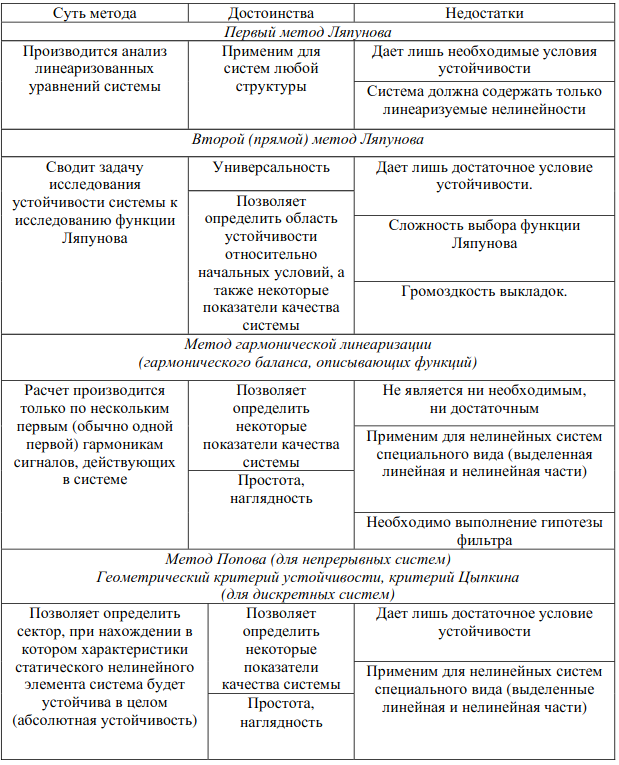
\includegraphics[scale=0.65]{Dissertation/images/DISSER-20.png}
    }
    \caption{Сравнительная таблица применения методов анализа устойчивости}\label{fig:Trel}
\end{figure}

Сравнительная таблица применения методов анализа устойчивости представлена на Рисунке~\cref{fig:Trel}.

\section{Выводы по главе}\label{sec:ch2/conc}

В данной главе решены следующие задачи:
\begin{enumerate}
    \item продемонстрирована математическая модель деревьев поддержки принятия решений и формулирования рекомендаций на основе нечеткого вывода Мамдани. Определены структура отображения входной и выходной информации, процесс обработки, фазификации и дефазификации наборов данных,
    \item разработан алгоритм модели поддержки принятия решений и формирования рекомендаций на основе прецедентов для задач принятия решений,
    \item продемонстрирована природа устойчивости обучения, рассмотренная, как отклонение в возмущениях в нелинейной адаптивной комбинированной системе с возмузением,
    \item продемонстрирована модель конъюнкционного вывода на основе нечетких функционалов принадлежности и работы деревьев поиска закономерностей,
    \item разработана модель формирования базы знаний, на основе таблицы ТРИЗ и семантического структурирования лексических термов, проведена работа по моделированию отображения графа в деревья закономерностей на основе аппроксимации эвристического отображения синтезом деревьев на основе критерия максимума взвешенной инофрмативности,
	\item проведен анализ конкурентных решений на рынке информационных технологий,
	\item систематизированы типы транзакционных моделей, 
	\item продемонстрирована постановка задачи проектирования архитектуры программного обеспечения, рассмотрены основные ограничения, допущения,
	\item продемонстрировано решение проблемы проектирования устойчивой архитетектуры автоматизированной системы управления,
	\item систематизирована информация по наиболее актуальным вопросам транзакционных проблем при проектировании архитектуры программного обеспечения автоматизированных систем управления.
\end{enumerate}

В результате каждая следующая закономерность стремится выделить наименее покрытые объекты, оказавшиеся наиболее трудными для предыдущих закономерностей. Это способствует повышению различности закономерностей, более равномерному покрытию объектов и повышению
обобщающей способности выпуклой комбинации закономерностей.

Перевыборка по отношению к выборке рассматривается как выборка по отношению к генеральной совокупности.
Важнейшим преимуществом бутстрапа являются:  
\begin{enumerate}
	\item простота реализации;  
	\item отсутствие необходимости гипотез о параметрах распределения данных;   
	\item возможность оценивания многих статистических характеристик (среднего, дисперсии, стандартного отклонения, доверительных интервалов, квантилей, коэффициентов корреляции и др.). 
\end{enumerate}

К недостатку метода можно отнести использование малореалистичного предположения о независимости перевыборок и значительные вычислительные затраты при их многократном построении. Метод оказывается особенно полезным, когда теоретическое распределение данных неизвестно или объем выборки мал для прямой статистической оценки.

\clearpage